\documentclass[11pt,a4paper]{article}
\usepackage[utf8]{inputenc}
\usepackage[T1]{fontenc}

\usepackage[dvipsnames,usenames]{color}
\usepackage[colorlinks=true,urlcolor=Blue,citecolor=Green,linkcolor=BrickRed]{hyperref}
\usepackage[usenames,dvipsnames]{xcolor}
\urlstyle{same}

\usepackage{amsthm,amsmath,amssymb,breqn}
\usepackage{fullpage}
\usepackage[ruled,noend,linesnumbered]{algorithm2e}     
\usepackage{enumerate,comment}
\usepackage{url}
\usepackage[capitalise]{cleveref}
\usepackage{todonotes}
\usepackage{tikz}
\usepackage[noadjust]{cite}
\usepackage{xspace}
\usepackage{graphicx}
\usepackage{float}
\usepackage{amsfonts}
\usepackage{color}
\usepackage{array}

%\pagestyle{plain}

\newcommand{\ceil}[1]{\left\lceil #1 \right\rceil}
\newcommand{\floor}[1]{\left\lfloor #1 \right\rfloor}
\newcommand{\poly}{\text{poly}}
\newcommand{\jump}{\text{jump}}

\newcommand{\Oh}{{O}}

% For cleverref compatibility
\newtheorem{theorem}{Theorem}[section]
\newtheorem{algo}{Algorithm}[section]
\newtheorem{corollary}{Corollary}
\newtheorem{lemma}{Lemma}
\newtheorem{observation}{Observation}
\newtheorem{fact}[theorem]{Fact}
\theoremstyle{definition}   
\newtheorem{definition}{Definition}
\usepackage{authblk}
\theoremstyle{remark}
\newtheorem{example}[theorem]{Example}
\newtheorem*{claim}{Claim}
\newtheorem{case}{Case}
\newtheorem{invariant}{Invariant}
\newtheorem{step}{Step}[section]

\newtheorem{property}[theorem]{Property}
\newcolumntype{R}[1]{>{\raggedleft\let\newline\\\arraybackslash\hspace{0pt}}m{#1}}

\begin{document}

\title{Dispersion on Trees\thanks{The research was supported in part by Israel Science Foundation grant 794/13.}}
\author[1]{Pawe\l{} Gawrychowski}
\author[1]{Nadav Krasnopolsky}
\author[2]{Shay Mozes}
\author[1]{Oren Weimann}
\affil[1]{University of Haifa, Israel}
\affil[2]{IDC Herzliya, Israel}


\date{}
\maketitle

\begin{abstract}
In the $k$-dispersion problem, we need to select $k$ nodes of a given graph so as to maximize
the minimum distance between any two chosen nodes. This can be seen as a generalization
of the independent set problem, where the goal is to select nodes so that the minimum distance
is larger than 1.
We design an optimal $\Oh(n)$ time algorithm for the dispersion problem on trees consisting
of $n$ nodes, thus improving the previous $\Oh(n\log n)$ time solution. 

We also consider the weighted case, where the goal is to choose a set of nodes of total weight at least $k$. We present an $\Oh(n\log^2n)$ algorithm improving the previous $\Oh(n\log^4 n)$ solution. Our solution builds on the decision version (where we know the minimum distance $\lambda$ between the chosen nodes) for which we present tight $\Theta(n\log n)$ upper and lower bounds. 
\end{abstract}

\section{Introduction}

\emph{Facility location} is a family of problems dealing with the placement of facilities on a network in order to optimize certain distances between the facilities, or between facilities and other nodes of the network. Facility location problems are usually if not always NP-hard on general graphs. There is a rich literature on approximation algorithms for general graphs (see e.g.~\cite{DavidB.Shmoys1997,Vazirani2003} and references therein) as well as exact algorithms for restricted graph families. In particular, many linear and near-linear time algorithms were developed for facility location problems on edge-weighted trees.   


In the most basic problem, called \emph{$k$-center}, we are given an edge-weighted tree with $n$ nodes and wish to designate up to $k$ nodes to be facilities, so as to minimize the maximum distance of a node to its closest facility. This problem was studied in the early 80's by Megiddo et al.~\cite{Megiddo1981} who gave an $\Oh(n\log^2n)$ time algorithm that was subsequently improved to $\Oh(n\log n)$ by Frederickson and Johnson \cite{Frederickson1983}. In the early 90's, an optimal $\Oh(n)$ time solution (also for more general variants such as placing facilities on any point along an edge) was given by Frederickson \cite{Frederickson1991a} using a seminal approach based on parametric search. 
%
A related problem, also suggested in the early 80's  \cite{Becker1982,Perl1981}, is \emph{$k$-partitioning}. In this problem the nodes have weight and we wish to delete $k$ edges in the tree so as to maximize the weight of the lightest resulting subtree. This problem was also solved by Fredrickson in $\Oh(n)$ time \cite{Frederickson1991} and also uses his parametric search framework. 
%
Finally, and the focus of this paper, is the  {\em $k$-dispersion} problem. In this problem we wish to designate $k$ nodes as facilities so as to maximize the distances among the facilities.  In other words, we wish to select $k$ nodes that are as spread-apart as possible. This can be seen as a generalization of the classical maximum independent set problem (that can be solved by binary searching for the largest value of $k$ for which the minimum distance is at least 2).  
%
It turns out that the $k$-dispersion and the $k$-partitioning problems are actually equivalent in the one-dimensional case (i.e. when the tree is a path).\footnote{The reduction simply creates a new path, whose edges correspond to nodes in the original path and vice versa. The original edge weights are now assigned to the nodes so we can run the $k$-partitioning solution.} However, such equivalence does not apply to general trees, on which $k$-dispersion seems more difficult than $k$-partitioning. In particular, until the present work, no linear time solution for $k$-dispersion was known. The fastest solution was the $O(n \log n)$ solution given in the early 90's by Bhattacharya and Houle \cite{Bhattacharya1991}. Bhattacharya and Houle also considered the case where nodes have weights and the goal is to select nodes with total weight at least $k$. For the weighted case, they gave an $\Oh(n\log^4 n)$ time solution. Both their solutions rely on the framework of Fredrickson.

\vspace{-0.1in}
\paragraph{Fredrickson's framework.}
Consider the $k$-dispersion problem. This optimization problem can be solved by repeatedly querying a {\em feasibility test} that solves the decision version of this problem. More formally, for a subset of nodes $P$ let $d(u,v)$ denote the distance between nodes $u$ and $v$ and let $f(P)=\min_{u,v\in P} \{d(u,v)\}$:


\begin{itemize} 
\item {\em The Dispersion Optimization Problem.} Given a tree with non-negative edge lengths, and a  number $k$, find a subset of nodes $P$ of size $k$  such that  $f(P)$ is maximized. 

\item  {\em The Dispersion Decision Problem.}  Given a tree with non-negative edge lengths, a number $k$, and a number $\lambda$, find a subset of nodes  $P$ of size $k$ such that  $f(P)\geq\lambda$. 
\end{itemize}

Bhattacharya and Houle designed a feasibility test that solves the decision problem in $\Oh(n)$ time. For completeness, we present a simplified version of it in Section~\ref{linear F.T.}.
%, improving on an earlier $\Oh(kn+n\log n)$ solution for single-path trees given by Wang and Kuo~\cite{Wang1988}. 
%We present a faster $\Oh(n\log^2 n)$ time algorithm. 
Using this feasibility test, the optimization problem can then be solved by parametric search: Since the answer is always
a distance between two nodes, we can construct an implicit representation of all possible $O(n^{2})$ distances and binary search over this representation. More precisely, the representation consists of $O(n)$ matrices that are each monotone in both row and columns. The total side length
of all the matrices is $O(n\log n)$, and we can provide constant-time access to any entry after $O(n\log n)$ preprocessing. Using $O(\log n)$ calls to such feasibility test we can solve the optimization problem in $O(n\log n)$ time. 
%
In this paper, we improve this to $O(n)$ by developing a feasibility test that requires {\em linear} preprocessing and can then be queried in \emph{sublinear} time. This was the approach of Fredrickson for $k$-partitioning and $k$-center. However, it turns out to be much more difficult for $k$-dispersion, and requires new ideas and techniques that we briefly describe next. Finally, for the weighted case, we present an $\Oh(n\log^2n)$ time solution for the optimization problem, and tight $\Theta(n\log n)$ upper and lower bounds for the decision problem. 

 

%ideas, at least at a high level. However, many details and tricks are actually different, and we believe
%that some of our techniques might be somehow simpler than his. 
%
%In particular, our algorithm is based on the (tweaked) micro-macro decomposition and the heavy path
%decomposition, which are both very standard data structure tools, instead of the less standard
%decompositions used by Frederickson.%TODO explain more?

\paragraph{Our feasibility test.}
We first define a variant of the well known micro-macro decomposition that partitions the input tree $T$ into $O(n/b)$ {\em fragments}, each containing $O(b)$ nodes and at most two {\em boundary nodes} incident to nodes in other fragments. Our variant is unique in the sense that it guarantees that one boundary node is always the root of the fragment (the other boundary node is called the {\em hole}). We use this to
 simulate a bottom-up feasibility test by jumping over entire 
fragments. I.e., knowing $\lambda$, we extend in $O(\log b)$ time a solution for a subtree of $T$ rooted at the framgment's hole to a subtree of $T$ rooted at the fragment's root. This is achieved by a rather complicated preprocessing which we next highlight.

The first step of the preprocessing computes values $\lambda_1$ and  $\lambda_2$ such that (1) there is no solution to the decision problem on $T$ for any $\lambda > \lambda_2$, (2) there is a solution to the decision problem on $T$ for any $\lambda \le \lambda_1$, and (3) for {\em most} of the fragments, the distance between any two nodes is either smaller than $\lambda_1$ or larger than $\lambda_2$. This is achieved with a recursive procedure that uses centroid decomposition in order to obtain the implicit monotone matrices required for Frederickson's parametric search. The (few) fragments that do not satisfy property (3) are handled naively in linear $O(b)$ time during query time. 

The fragments that do satisfy property (3) are handled in the second step of the preprocessing: The goal here is to eliminate from such fragments nodes that are guaranteed to be included or excluded from an optimal solution for any $\lambda \in [\lambda_1,\lambda_2)$. This is done by looking at the path from the hole to the root of the fragment and running the linear-time feasibility test for all subtrees hanging off from it (all contained in the fragment). It turns out that we can run this feasibility test without knowing $\lambda$ as long as we can determine for any two nodes if their distance is smaller than $\lambda_1$ or larger than $\lambda_2$ (which we can, in constant time). This allows us to conceptually trim the fragment and think of it as a caterpillar. The spine of the caterpillar is the hole-to-root path and each spine node has two leaf children - a \emph{certain} node (that is guaranteed to be included in an optimal solution for any $\lambda$, and a \emph{candidate} node (whose inclusion in an optimal solution depends on $\lambda$). Finally, we perform additional pruning of some caterpillar leaves that results in a highly structured caterpillar where the leaves are in monotonically increasing distance from both the hole and the root. This structure enables us to precompute for each candidate node, assuming this node is the bottom-most node in the solution, what are all the other nodes in the solution. Upon query, we can then jump over the entire fragment  in $O(\log b)$ time by binary searching for this bottom-most node. 

The above feasibility test is presented in Section~\ref{sublinear f.t.}. By appropriately setting up $b$ to balance the preprocessing and the query time, the overall preprocessing time is $O(n\log\log n)$. The bottleneck of this preprocessing are its calls to the vanilla linear-time feasibility test.  
In Section~\ref{sectionlog*} we improve this gradually to $O(n\log^* n)$ by constructing a sequence of faster and faster feasibility tests. 
We iteratively use the current feasibility test to construct the next (faster) feasibility test.
Every iteration uses an appropriately chosen parameter $b$ for the micro-macro decomposition
as to guarantee that the construction time is $O(n)$. The parameters grow exponentially,
so after $O(\log^{*}n)$ iterations we obtain a feasibility test with sublinear query and $O(n\log^* n)$ preprocessing. 

Finally, in Section~\ref{sectionLinear}, we improve the preprocessing from $O(n\log^* n)$ to $O(n)$. This means we cannot afford to construct each micro-macro decomposition separately. We overcome this by making each decomposition a refinement of the previous one. This requires relaxing the decomposition so that a fragment may contain more than $O(b)$ nodes. 
We believe that this simple micro-macro variant is of independent interest. 
%
The main difficulty remaining is how to preprocess the fragments. We cannot afford to touch very node of every fragment at every decomposition level. Therefore, we take a closer look at how a (large) fragment decomposes into smaller fragments. 
We show that a large fragment can be reduced to a concatenation of small caterpillars, each corresponding to a small fragment that we have already preprocessed. We then very carefully tailor these small fragments while reusing the results of their preprocessing. We show that this tailoring amortizes to $O(n)$ over all decompositions. This turns out to be quite technical. 


\section{A Linear Feasibility Test}\label{linear F.T.}
%\begin{algo} \label{unWeightedFeasibilityAlgo}
We show a recursive linear algorithm. At each step of the recursion, we would like to provide a valid solution with maximal cardinality for the current subtree, given some $\lambda$, i.e. the algorithm will maintain the following invariant:
\begin{invariant}\label{Maximality of P and distance of closest node invariant}
For every node of the tree, $r$, the algorithm produces $P$, a subset of the vertices of the subtree rooted at $r$, s.t. $f(P)\geq\lambda$ and $|P|$ is maximal. Out of all such valid subsets with maximal cardinality, the distance between $r$ and the node closest to it is maximized in $P$.
\end{invariant}
In each step we are given a root vertex $r$, its children nodes $r_{1},r_{2},...,r_{k}$, and for each child we are given a maximal valid solution for the feasibility test on its subtree. We would like to produce a maximal valid solution for the feasibility test on $r\text{'s subtree}$.
Denote by $P_{1},...,P_{k}$ the solutions for the feasibility test on each subtree rooted at a child of $r$.
\begin{definition}
For any subtree of $T$ rooted at node $r$, and a valid solution $P$ for a feasibility test on the subtree (i.e. $f(P)\geq\lambda$), we call a node $u\in P$, s.t. $d(r,u)<\frac{\lambda}{2}$, the \emph{candidate} node of the subtree (or a candidate with respect to $r$). We call the vertices in $P$ that are not the candidate (i.e. every node $v \in P$ s.t. $d(r,v)\geq \frac{\lambda}{2}$), \emph{certain} (w.r.t $r$). When it is clear from the context, we will not explicitly mention which subtree we are referring to.
Note that for any vertex $x$, a valid solution to the feasibility test on $T_x$ contains at most one candidate vertex.
\end{definition}

\paragraph{The recursion step.} Given $P_{1},...,P_{k}$, we would like to produce a solution for $r$'s subtree.
\begin{enumerate}
\item Put in $P$ all the vertices in $P_{1},...,P_{k}$, except for the candidate vertices.
\item Take all candidate nodes $u$ s.t. $d(u,r) \geq \frac{\lambda}{2}$ (i.e. they are certain w.r.t $r$).
\item If it exists, take $u'$, the candidate node farthest from $r$ s.t. $d(u',r) < \frac{\lambda}{2}$ and $d(u',x)\geq \lambda$, where $x$ is the closest node to $u'$ we have chosen so far.
\item Check if it is possible to take $r$ into the solution by looking at the closest vertex to it we have already put in $P$. If possible, put $r$ in the solution.
\end{enumerate}
Iterating over the input tree bottom-up as described, will provide us with the solution to the Dispersion decision problem as the output for the root of the tree.

\paragraph{Proof of correctness.}
We shall now prove the correctness of the algorithm. We will do this by proving that Invariant \ref{Maximality of P and distance of closest node invariant} holds for every step of the algorithm.

Let us observe some node of the tree $r$, and prove that the invariant holds for it, assuming that it holds for its children, $r_{1},r_{2},...,r_{k}$. Denote the subtree rooted at a node $x$ by $T_x$. Assume for contradiction that $P'$ is a subset of the vertices of $T_r$, s.t. $f(P')\geq\lambda$ and $|P'| > |P|$. Let us look at the two possible cases:
\begin{enumerate}
\item \textbf{\boldmath$P'$ has more certain nodes w.r.t \boldmath$r$ than \boldmath$P'$}: All certain nodes w.r.t $r$, are in subtrees rooted at children of $r$, and so there must be some child of $r$, $r_i$, s.t. $P'_{r_i}$ has more certain nodes w.r.t $r$ than $P_{r_i}$ (where $P'_{r_i}$ is $P'$ restricted to $T_{r_i}$). This can only be if $|P'_{r_i}| > |P_{r_i}|$, or if the closest node to $r_i$ in $P'_{r_i}$ is farther than the closest node in $P_{r_i}$, and so the invariant does not hold for $r_i$.
\item \textbf{\boldmath$P'$ has the same number of certain nodes w.r.t \boldmath$r$ as \boldmath$P$, but \boldmath$P'$ has a candidate w.r.t \boldmath$r$  and \boldmath$P$ does not}: Denote the candidate node of $P'$ by $u$. We have two possible cases. First, if $u=r$, then there is some node $v \in P$ s.t. $d(u,v)<\lambda$. Assume that $v$ is in the subtree rooted at $r_i$. In this case, either $|P'_{r_i}|=|P_{r_i}|$ and the closest node to $r_i$ in $P'_{r_i}$ is farther than the closest node in $P_{r_i}$, and the invariant does not hold for $r_i$, or $|P'_{r_i}|<|P_{r_i}|$ and so there must be some $r_j$ s.t. $|P'_{r_j}|>|P_{r_j}|$, and the invariant does not hold for $r_j$. Second, if $u$ is in one of the subtrees rooted at children of $r$, since all certain nodes w.r.t $r$ are also in these subtrees, there must be one such subtree, $r_l$ s.t. $|P'_{r_l}| > |P_{r_l}|$, and so the invariant does not hold for it.
\end{enumerate} 
Thus we have proven that $P$ is of maximal cardinality. Now, assume for contradiction that $P'$ is a subset of the vertices of the subtree rooted at $r$, s.t. $f(P')\geq\lambda$ and $|P'| = |P|$, but the closest node to $r$ in $P$ (denoted by $u$) is closer to $r$ than the closest node to $r$ in $P'$. Assume that $u \neq r$ and denote by $T_{r_i}$ the subtree that $u$ is in. Thus, either $|P'_{r_i}| = |P_{r_i}|$, but the closest vertex to $r_i$ in $P'_{r_i}$ is farther away from $r_i$ than $u$, which means the invariant does not hold for $T_{r_i}$, or $|P'_{r_i}| < |P_{r_i}|$, and it makes up for it in some other subtree where the invariant does not hold. If $u=r$, then since $|P'| = |P|$, there must some child of $r$, $r_i$, s.t. $|P'_{r_i}| > |P_{r_i}|$, and so the invariant does not hold for $r_i$. We have proven that Invariant \ref{Maximality of P and distance of closest node invariant} holds for every node of the input tree, and thus proven the correctness of the algorithm.
%TODO write that this is enough for an O(nlogn) solution

\section{A Sublinear Feasibility Test with \boldmath
$O(n\log\log n)$ Preprocessing}\label{sublinear f.t.}
The main idea here is partitioning the input tree into fragments and preprocessing them, so that in query time we can process fragments in sub-linear time. For this, we need to use a partitioning with some specific attributes, which we now present. We assume the tree is binary, and justify this assumption later.
\subsection{Tree partitioning}\label{tree partitioning}
We would like to partition the tree into fragments s.t. each fragment will be connected to the rest of the tree by at most two vertices. Each fragment will have at most $O(b)$ vertices, and there will be at most $n/b$ fragments. Each fragment is defined by its border vertices $u$ and $v$, s.t. $v$ is a descendant of $u$. The fragment will consist of $u$'s subtree without $v$'s subtree ($v$ itself is not part of the fragment). We call the path from $u$ to $v$, the fragment's \textit{spine}, and $v$'s subtree the \textit{hole} of the fragment. In the case where the fragment has only one border vertex, i.e. the fragment is a subtree of the input tree, we say the fragment has no hole. We call such a partition of the tree a \emph{good partition}.

\begin{figure}
\begin{center}
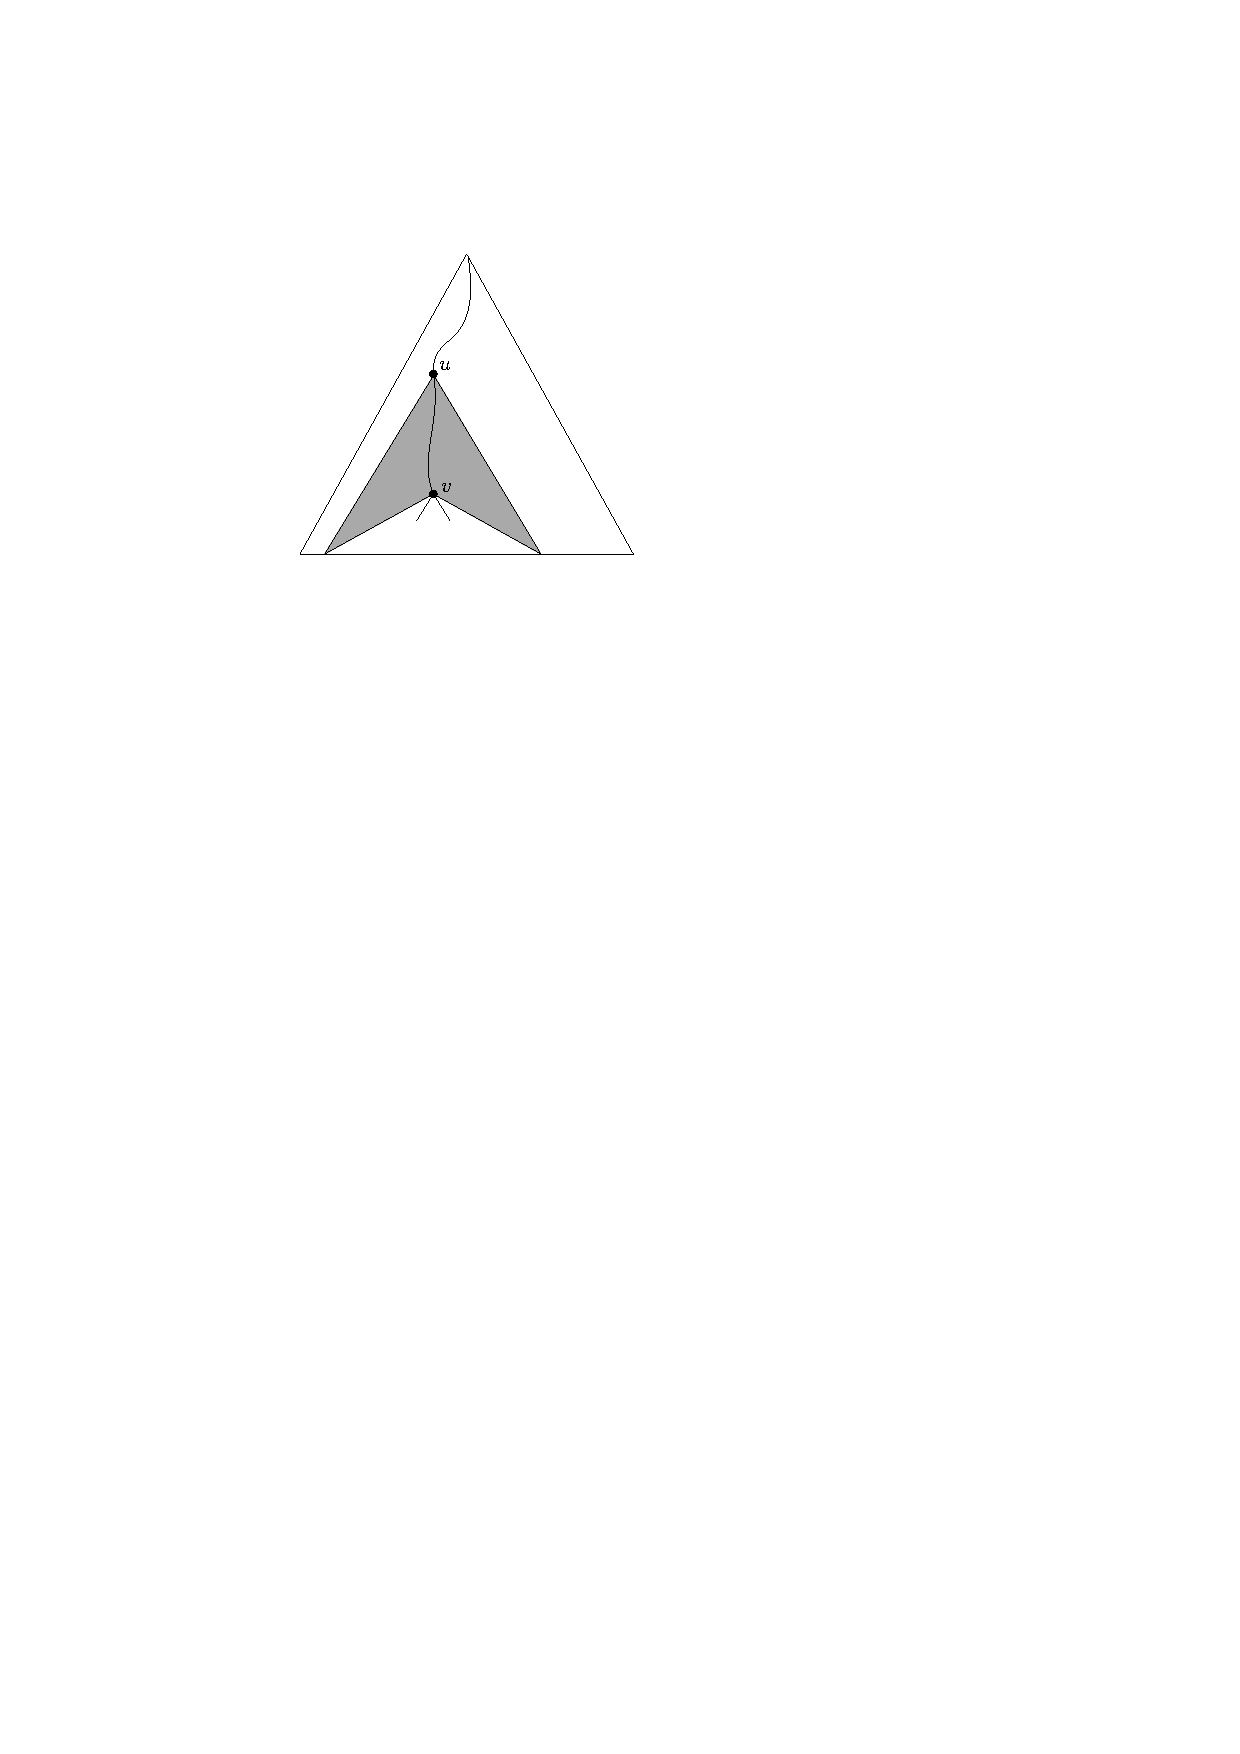
\includegraphics[scale=0.7]{fragment}
\end{center}
\caption{Example of a fragment in a good partition. The fragment consists of the subtree of $u$ without the subtree of $v$. We call $u$ the \emph{root} of the fragment and $v$ the \emph{hole} of the fragment. The path from $u$ to $v$ is called the \emph{spine} of the fragment.}
\end{figure}

\begin{lemma}\label{basic partitioning lemma}
For any binary tree on $n$ nodes and a parameter $b$, there is a good partition of the tree.
\end{lemma}
\begin{proof}
We prove the lemma by construction. Call a node \textit{large} if the size of its subtree is at least $b$
and \textit{small} otherwise. Consider the tree $T_L$ induced by the large nodes of the original tree. 
For each leaf $u\in T_{L}$, we make each of its children in the original tree a new fragment with no holes.
Each leaf of leaf of $T_{L}$ is the root of a subtree of size at least $b$ in the original tree, and these subtrees
are all disjoint, so we have at most $n/b$ leaves in $T_{L}$. Each of them creates up to two fragments
since the tree is binary, and each of these fragments is of size at most $b$ by definition.
The natural next step would be to keep cutting of maximal fragments of size $b$ from the remaining
part of the tree. This does not quite work, as we might create fragments with multiple boundary
nodes with such a method.
Therefore, the next step is to consider every branching node in $T_{L}$ instead, and make it a fragment
consisting of just one node. This also creates up to $n/b$ fragments, since in any tree the number of
branching nodes is at most the number of leaves.
Ignoring the already created fragments, we are left with large nodes that form unary chains in $T_{L}$.
Each of these nodes might also have an off-chain child that is a small node. We have at most $n/b$ of these chains
(because each of them corresponds to an edge of a binary tree on at most $n/b$ leaves).
We scan each of these chains bottom-up and greedily cut them into fragments of size at most $b$.
Denoting the size of the $i$-th chain by $b_{i}$, the number of fragments created in this phase is
bounded by $$\sum_{i=1}^{n/b} \left\lceil \frac{b_i}{b} \right\rceil = O(n/b).$$
In total we have created $O(n/b)$ fragments, and each of them is of size at most $b$.
By adjusting $b$ we can obtain up to $n/b$ fragments, each of size $O(n)$.
\end{proof}
This partitioning is done in $O(n)$ time.

\subsection{Preprocessing fragments} \label{Pre-Processing Fragments}
We now would like to preprocess the fragments s.t. we can later check in constant time for any two nodes in a fragment, $u_1$ and $u_2$, if $d(u_1,u_2)\geq\lambda$, and if $d(u_1,u_2) \geq \frac{\lambda}{2}$, for any possible $\lambda$. The possible values of $\lambda$ in the beginning are of course all the pairwise distances in the input tree. We achieve the ability to perform such queries for most of the fragments, by using a parametric search method by Frederickson that allows us to eliminate some of the possible values of $\lambda$, using our existing feasibility test. By the end of this elimination process, most of the fragments will have the property that any pairwise distance inside them is either smaller then the smallest possible value of $\lambda$ or
 greater or equal to the largest possible value of $\lambda$. The same will hold for $\frac{\lambda}{2}$.
For each fragment, we will implicitly construct matrices of total side length (number of rows and columns) $O(b \log b)$, that are row and column sorted, and contain all pairwise distances in the fragment.

\begin{definition} \textbf{Centroid Decomposition}
A node $v\in T$ is a centroid if every connected component of $T\setminus\{v\}$ consists of at most $\frac{|T|}{2}$
nodes. The centroid decomposition of $T$ is defined recursively by first choosing a centroid $v\in T$
and then recursing on every connected component of $T\setminus\{v\}$ called \emph{pieces}.
\end{definition}

\begin{figure}
\begin{center}
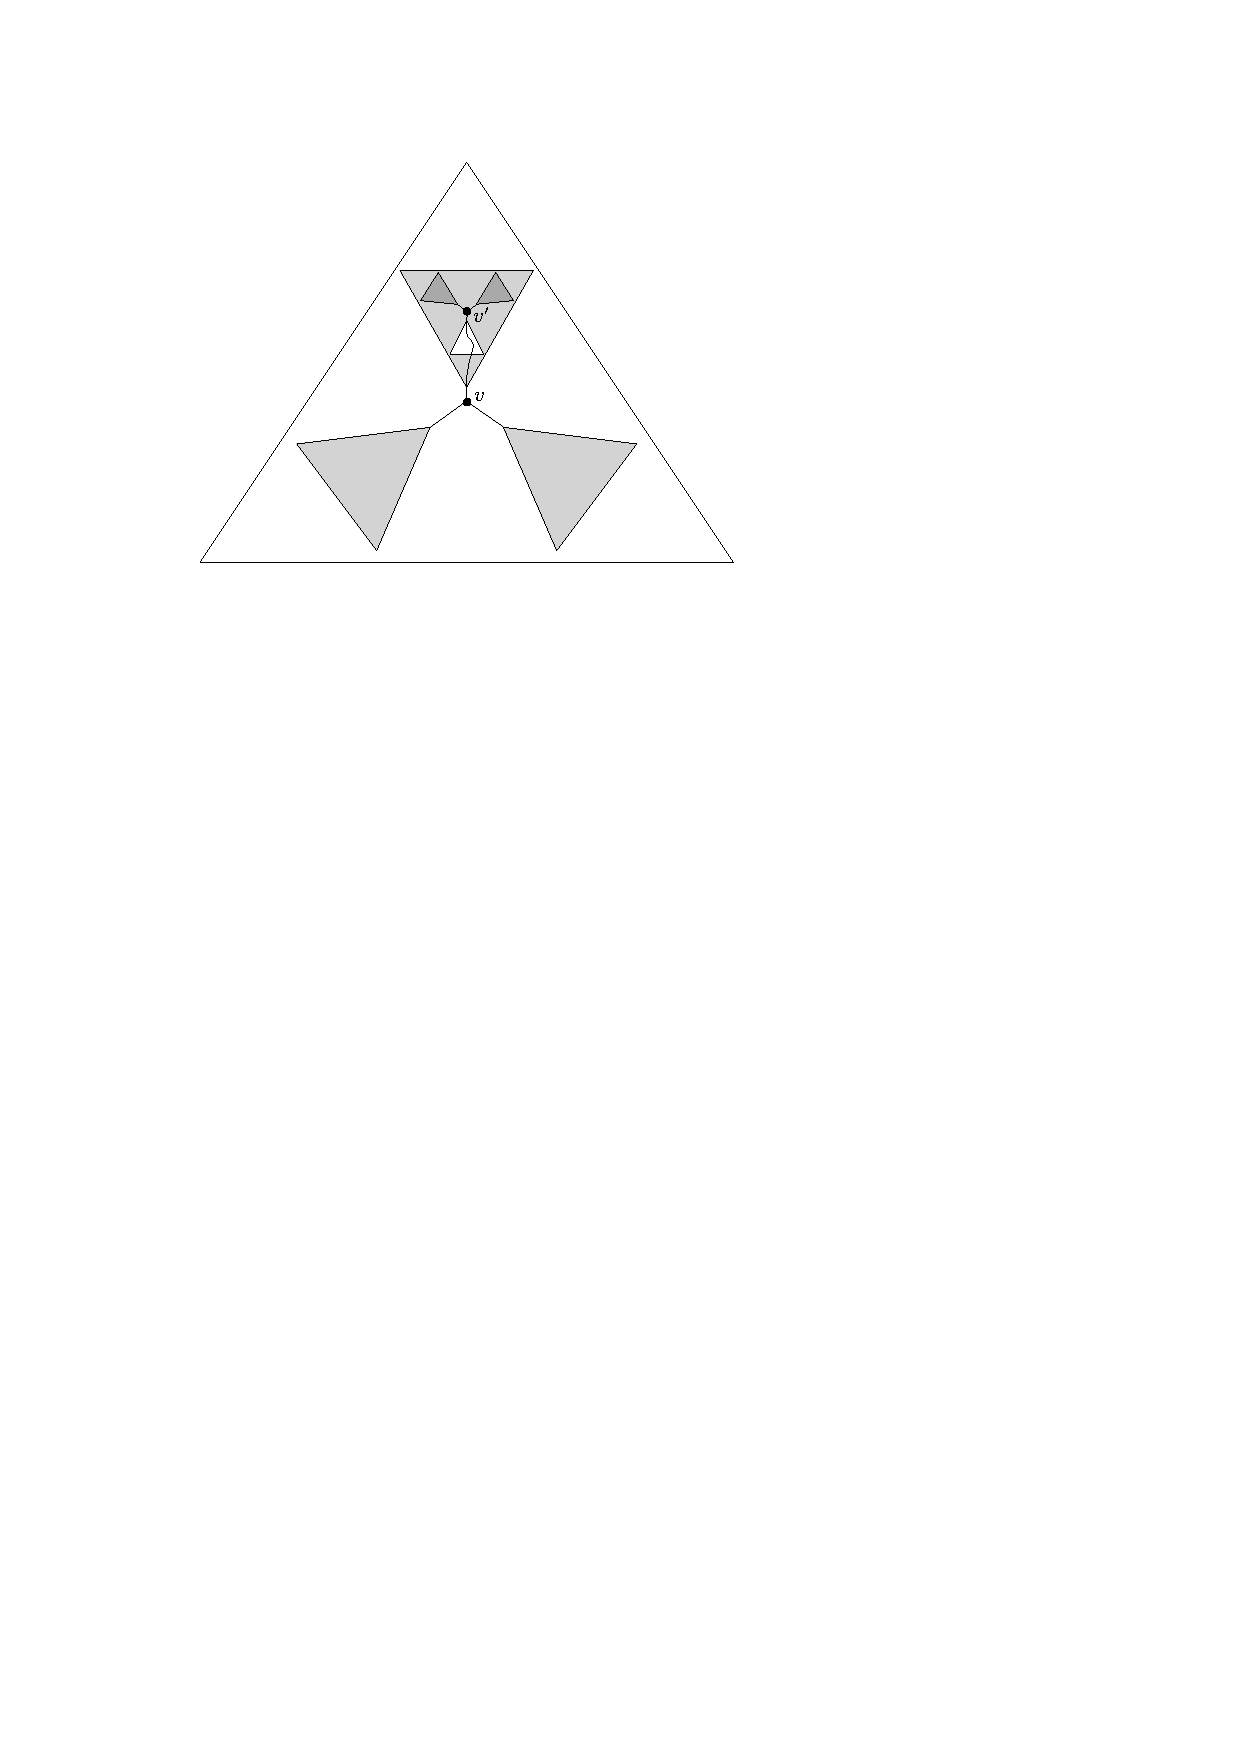
\includegraphics[scale=1]{centroid}
\end{center}
\caption{A single step in the centroid decomposition. Removing $v$ splits the tree into three pieces, s.t. none of them has more than $\frac{n}{2}$ nodes. The white piece is problematic, since the paths from its nodes to $v$ do not pass through the inner centroid $v'$.}
\end{figure}

Apply the centroid decomposition on each fragment. This take linear time. Since we assume our input tree is binary, the centroid at each level of the recursion will split the tree into three pieces. Now, run the following recursive routine: at each level of the recursion, we are given the three pieces of the decomposition, and for each of them a sorted list of the distances to their inner centroid. We would like to compute a sorted list of distances of the nodes in all three pieces, to the current centroid. This would give us the ability to compute, in constant time, the distance between any two nodes that are in different pieces (since the path between them goes through the centroid). Let us look at one of the three pieces we have already processed. It contains three pieces of its own. For two of these pieces, it holds that the path from every node inside them to the outer centroid passes through the inner centroid. We call the third piece, for which this does not hold a \textit{problematic} piece. For the two pieces that are not problematic, we can add to all the entries of the lists we have, the distance from the inner centroid to the outer centroid, and then merge the two sorted lists. This is all done in linear time.

Our only problem now is the piece where the paths to the outer centroid do not go through the inner one. But notice that if we go one step deeper in the recursion we can see that inside the problematic piece there are two pieces that are not problematic, as the paths from all their nodes to the outer centroid pass through their inner centroid. We can do the same kind of merging for their two list, and then look deeper inside the remaining problematic piece, and so on. This recursive routine will also take linear time. Altogether we have $O(\log b)$ levels of recursion, and spend linear time on each one, so we get a running time of $O(b \log b)$ per fragment. For now, we set $b$ to $\log ^2 n$ and get a running time of $O(\frac{n}{b} \cdot b\log b) = O(n \log \log n)$ for all fragments.

Now we have for level $i$ of the recursion $3^i$ centroids, and for each of them a sorted list of the distances to all nodes in the appropriate pieces. We can find any pairwise distance in a piece by adding two entries of this list. Since the lists are sorted, we can look at the situation as if we have $3^i$ matrices of and their total side length is $n$ \footnote{We cannot actually afford to explicitly store these matrices, but that is not needed.}. The matrices from all levels of the recursion, contain all the pairwise distances inside all the fragments. Note that we also have some entries in the matrices that do not actually represent pairwise distances in the tree, because some entries in the matrix represent the length of a path between two nodes that passes through the centroid of the piece, but the shortest path between these two nodes does not pass through the centroid. This does not matter, since it just means we will do some unnecessary eliminations.

Now, we can use a parametric search algorithm by Frederickson to eliminate entries of the matrices. The idea of this method is looking at specific locations in the matrices, running feasibility tests on their values, and eliminating large pieces of the matrices. This is possible because these matrices are both row and column sorted, and because if some number $x$ is not a feasible solution for the dispersion problem, then any number $y>x$ is also not feasible, and also, if $x$ is feasible, then any number $z<x$ is also feasible. Using this searching method, we find the interval of possible solutions to the dispersion optimization problem\footnote{The possible solutions to the dispersion optimization problem are all the pairwise distances in the input tree. All of these distances are represented in entries of the matrices we have implicitly constructed.}, $[\lambda_1,\lambda_2)$, s.t. the $\lambda^*$ we are searching for is in this interval, $\lambda_1$ is the largest number we know is feasible, and $\lambda_2$ is the smallest number we know is not feasible. We call fragments that do not contain a pairwise distance that is in the interval \textit{inactive}, and all other fragments \textit{active}. Since we would like to also answer queries for $\frac{\lambda}{2}$, we do the same process for matrices that contain twice the distance in every entry of the original matrices.
For this search, we use the following theorem of \cite{Frederickson1991}:
\begin{theorem}[\cite{Frederickson1991}]\label{Frederickson's theorem}
Let $M$ be a collection of $N$ sorted matrices ${M_l, M_2, . . . , M_N}$ in which matrix $M_j$ is of dimension $m_j \times n_j$, $m_j \leq n_j$, and $\sum_{j=1}^{N} m_j = m$.
Let p be nonnegative. The number of feasibility tests needed to discard all but at most p of the elements is $O(\max \lbrace \log(\max_{j} \lbrace n_j \rbrace), \log(\frac{m}{p+1}) \rbrace)$, and the total running time exclusive of feasibility tests is $O(\sum_{j=1}^{N} m_j \cdot \log (2n_j/m_j))$.
\end{theorem}
In our case $m=b \log b \cdot \frac{n}{b} = n \log b$ (since for each of the $\frac{n}{b}$ fragments, we have $\log b$ levels of the centroid decomposition, and at each level we have the distance of every node to a centroid) and we set $p$ to be $n/b^2$. The theorem implies that we can use $O(\log b)$ feasibility tests and discard all but $n/b^2$ elements of the matrices. We also pay $O(n \log b)$ exclusive of the feasibility tests. This means that we have at most $n/b^2$ active fragments (out of all $n/b$ fragments). 

For inactive fragment, it is clear that we can now answer queries checking whether some pairwise distance inside the fragment is at least $\lambda$, or if it is less than $\frac{\lambda}{2}$ \footnote{We can easily compute any pairwise distance in the tree in $O(1)$ time by precomputing all distances to the root of the tree, and using LCA queries \cite{Bender2000}, \cite{Djidjev1991}.}.

Active fragments will be processed as in the linear algorithm described before, so we can ignore them for now. We refer to the certain node which is closest to the root simply as \textit{the certain node}. We now do the following preprocessing for each inactive fragment:
\begin{enumerate}
\item\textbf{Reduce the fragment to a caterpillar:}\\
Observe that each fragment is comprised of its spine, and the subtrees hanging off of it. Using queries on pairwise distances as described above, we can use our linear feasibility test on the subtrees hanging off the spine, and get a candidate and a certain node for each of them. This is done in linear time.
Our fragment is now reduced to a caterpillar with at most leaves attached to each spine node: a candidate
node and a certain node.
\item\label{removing certain nodes}
\textbf{Find the candidate nodes that will certainly not be taken:}\\ %TODO add drawing
Let the $i$-th leaf of the caterpillar be connected by an edge of length $y_i$ to a spine node at distance $x_i$ from the root of the caterpillar. Order the leaves so that $x_1 < x_2 < ... < x_k$.
Some of the candidate nodes can be ignored as they "collide" with certain nodes. We start by finding the closest certain node to each candidate node. We can do this in linear time by scanning the caterpillar bottom-up, while saving for each candidate node, the closest certain node below it and the distance to it. We then do the same scan from top to bottom, and from both scans combined, we get for each candidate node the closest certain node and the distance to it. Now we want to find the candidate nodes that are too close to a certain node. We can do this since we are looking at an inactive fragment, and so a pairwise distance in it must be either smaller than $\lambda_1$ or greater or equal to $\lambda_2$. Delete all candidate nodes for which the distance to the closest certain node is smaller than $\lambda_1$. 
Now we are only left with some of the candidate nodes to consider, and for all of them it hold that $y_i < \frac{\lambda_1}{2}$ (otherwise they would be certain), and from now on we can ignore the certain nodes.
\item\label{making distances from the root monotone}
\textbf{Prune the caterpillar so that the leaves' distances to the root are non-decreasing:}\\
Consider the $i$-th leaf, $u_i$, and the adjacent leaf above it, $u_{i-1}$. See Figure~\ref{fig:pruning}. Suppose that $u_{i-1}$ is farther from the root than $u_i$ (i.e. $x_{i-1}+y_{i-1} > x_i+y_i$), then:
$$ d(u_{i},u_{i-1}) = x_i-x_{i-1}+y_i+y_{i-1} = x_{i} + y_{i} - x_{i-1} + y_{i-1} < 2y_{i-1} < \lambda_1.$$
So an optimal solution cannot contain both $u_{i}$ and $u_{i-1}$. We claim that if the solution contains
$u_{i}$ then it can be replaced with $u_{i-1}$. To prove this, it is enough to argue that
$u_{i-1}$ is farther away from any node above it than $u_i$, and $u_i$ is closer to any node below it than $u_{i-1}$.
Consider a node $u_{j}$ that is above $u_{i-1}$ (so $j<i-1$), then:
$$d(u_j,u_{i-1}) - d(u_j,u_{i}) = y_{i-1}-(x_i-x_{i-1})-y_i = x_{i-1}+y_{i-1}-(x_i+y_i) > 0.$$
Now consider a node $u_{j}$ that is below $u_{i}$ (so $j>i$), then:
$$d(u_j,u_{i-1}) - d(u_j,u_{i}) = y_{i-1}+(x_i-x_{i-1})-y_i > 2(x_i-x_{i-1}) > 0.$$
So in fact, we can remove the $i$-th leaf from the caterpillar if $x_{i-1}+y_{i-1} > x_i+y_i$. 
We traverse the caterpillar from bottom to top and decide if the current leaf $u_{i}$ should be removed.
To this end, it is enough to compare its distance to the root with the most recently processed non-removed leaf,
so the whole scan takes linear time in the number of candidate nodes. In the end, the distances of the
remaining leaves from the root are non-decreasing.

\begin{figure}
\begin{center}
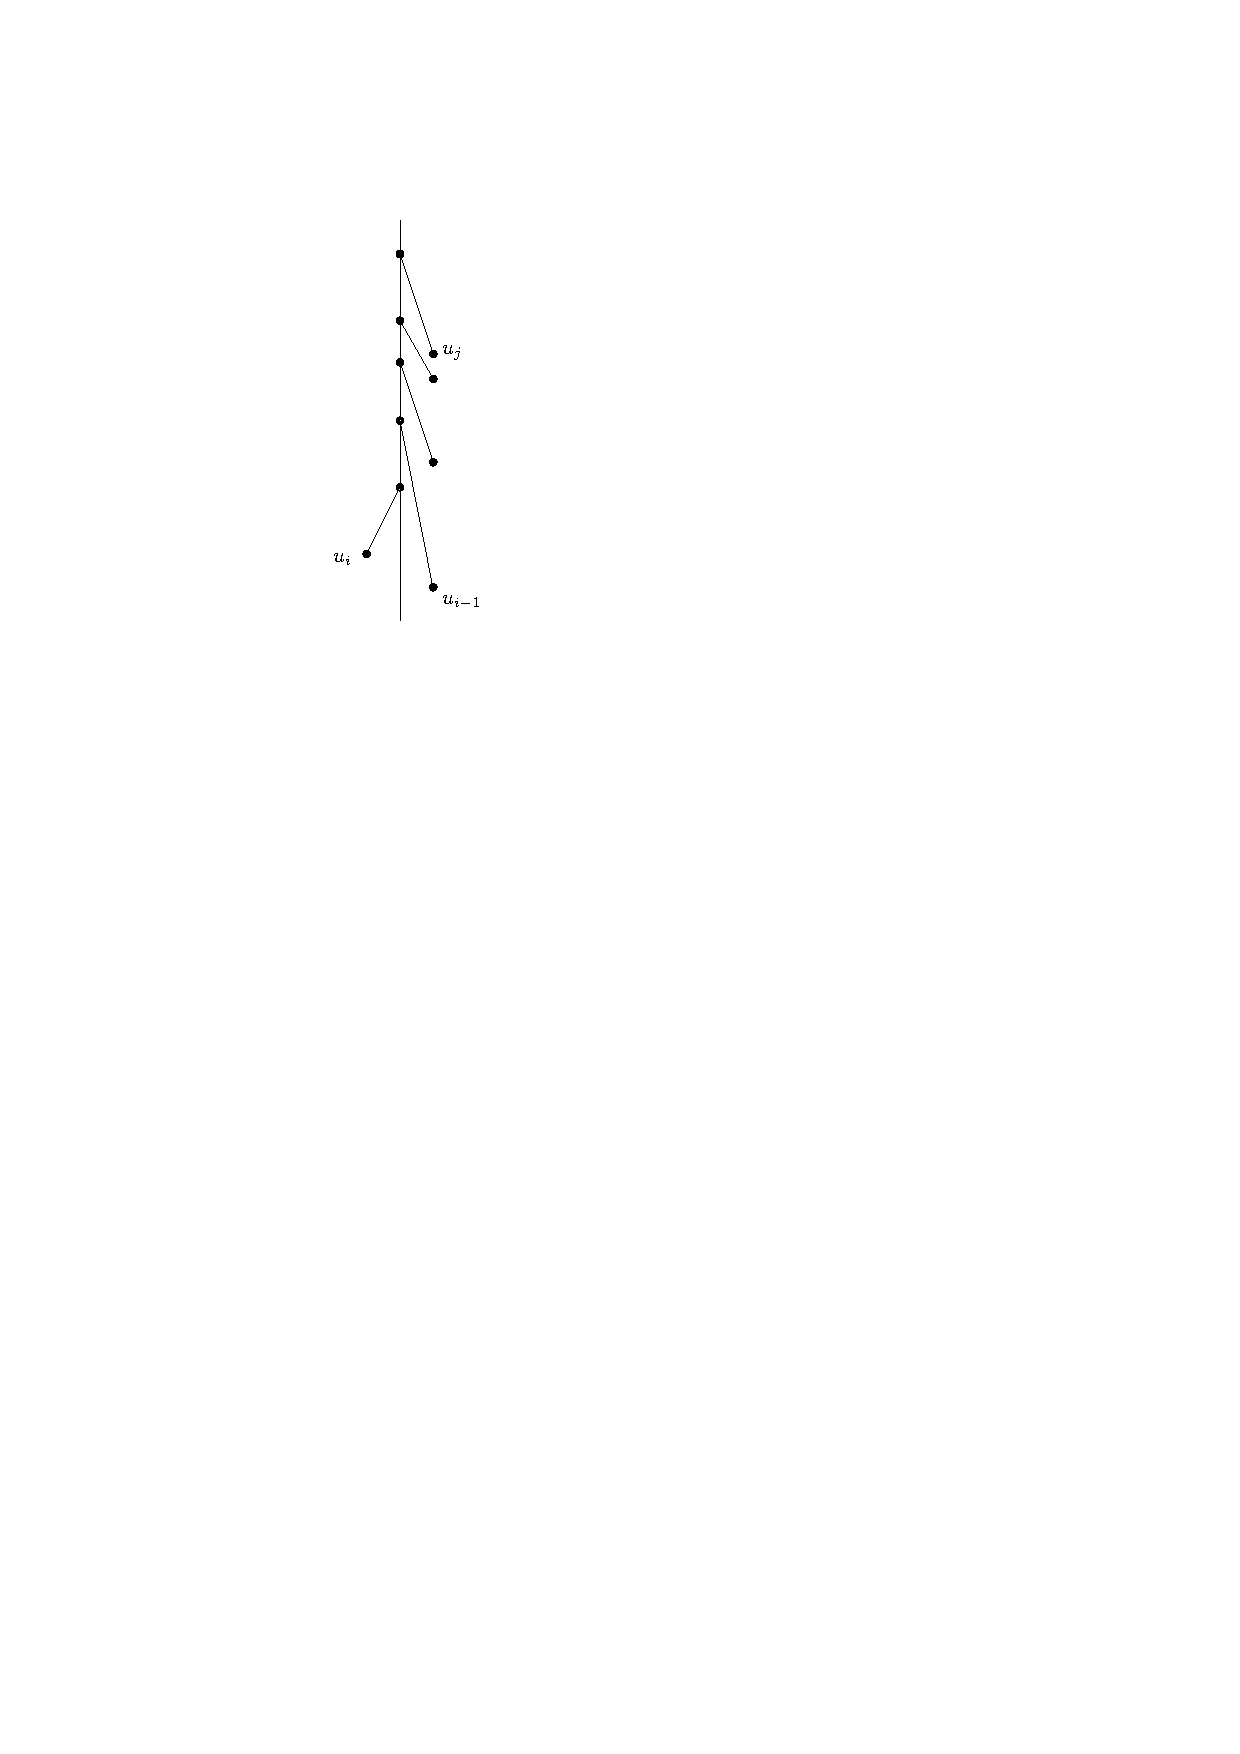
\includegraphics[scale=0.5]{caterpillar}
\end{center}
\caption{Pruning the caterpillar so that the distances of leaves from the root are non-decreasing: If $d(u_i,r)<d(u_{i-1},r)$ then  we can remove $u_{i}$ since (1) an optimal solution cannot contain both $u_{i}$ and $u_{i-1}$ (the distance between them is too small), and (2) if an optimal solution contains $u_{i}$ then it can be replaced with $u_{i-1}$ (every leaf $u_j$ is farther from $u_{i-1}$ than from $u_i$). \label{fig:pruning}}
\end{figure}

\item \label{making distances from the hole monotone}
\textbf{Prune the caterpillar so that the leaves' distances to the hole are non-decreasing:}\\
This is done as in the previous step.
\item\textbf{Compute the solution for any possible distance of the hole's candidate node:}\\
In query time we want to process each fragment after its hole has already been processed.
We call a set of consecutive leaves of the caterpillar, that contains the closest leaf to the hole, a \emph{suffix} of the caterpillar. Similarly we can define the caterpillar's \emph{prefix}.
Assuming we know what is the closest chosen node in the fragment's hole, we can eliminate an entire suffix of the caterpillar (because of the monotonicity of the distances of candidate nodes from the hole). We can compute in preprocessing, for any possible eliminated suffix, which nodes in the fragment should be chosen, and also which nodes are the candidate and certain node we need to pass to the next fragment.
In order to precompute this, scan the caterpillar from top to bottom. For every possible prefix of the caterpillar we would like to store the numbers of nodes chosen, the certain node and the candidate node, assuming all nodes that are not in the prefix are eliminated as they are too close to the hole. Consider the bottom node of the current prefix. If the distance of this node to the fragment's root is less than $\frac{\lambda}{2}$\footnote{We do not actually know $\lambda$ in preprocessing, but due to the previous steps, such a query of a node inside the fragment would produce the same result for any possible $\lambda$.}, store it as the candidate node, zero as the number of chosen nodes, and NULL as the certain node (if this fragment has a hole, we will consider its candidate and certain node in query time). Else, (the node's distance to the root is greater or equal to $\frac{\lambda}{2}$), write it as the certain node. Then, use binary search to find the closest node above it, that is at distance of at least $\lambda$. Add 1 to the number of chosen nodes stored in the node we found, and either store it as the candidate node, or copy the candidate node stored there. This would take $O(b \log b)$ time. We can improve this by not binary searching for the first node far enough, but instead saving it for each prefix, and then only going down from the previous node found. This would only take $O(b)$ time.
\end{enumerate}

\subsection{Feasibility test}
We now scan the whole tree, and for each inactive fragment we would like to produce in $O(\log b)$ time: the number of chosen nodes in the fragment, the candidate node, and the certain node. In this procedure we use the caterpillars we have created in the preprocessing. We run this procedure bottom-up, so we assume that the fragment rooted at the hole of the current one has already been processed. Notice that now we are given $\lambda$. Denote the root of the fragment by $r$, and the current fragment's leaf which is farthest from $r$, by $v$.

If the hole does not have a candidate node, denote its certain node by $u$. We compute the suffix of the fragment that cannot be taken. We can do this by binary searching for the first node of the fragment that is at distance at least $\lambda$ (which is given now) from $u$. We have precomputed all we need to know once we have the relevant prefix (i.e. the nodes we choose in the current fragment, including the certain and candidate nodes).

If the hole does have a candidate node, denote it by $u$. Assume $d(u,v) \geq \lambda$, then $u$ does not eliminate any suffix of the current fragment (due to the monotonicity of distances from the hole). Thus, we can take the nodes chosen so far, including the hole's candidate, $u$, and add to them the nodes we stored in preprocessing for the case that no suffix is eliminated. If $u$ and $v$ "collide" (i.e. $d(u,v) < \lambda$), we have the following two cases:
\begin{enumerate}
\item $d(r,v) > d(r,u)$: In this case, $v$ is farther from the root than $u$, which is possible since the monotonicity only holds inside each fragment. In this case we do not take $u$ into the solution, and only take the certain nodes we have so far. Because any certain node does not "collide" with $u$, it is also far enough from $v$, and so no suffix is eliminated and we take the appropriate nodes from the current fragment.
\item $d(r,v) \leq d(r,u)$: In this case we need to consider the suffixes of the current fragment, as in the case where the hole does not have a candidate.
\end{enumerate}
Each feasibility test costs us $O(\log b)$ for each inactive fragment, and $O(b)$ for each active one. In total $O(\frac{n}{b} \cdot \log b) + O(\frac{n}{b^2} \cdot b) = O(\frac{n \log \log n}{\log ^2n})$.


\subsection{\boldmath$O(n\log\log n)$ Preprocessing} 
The general idea of the algorithm is to use the heavy path decomposition. We are searching for $\lambda^*$, which is the distance between some two nodes in the tree, and the largest number for which a feasibility test would return true.
\begin{definition}
\emph{Heavy Path Decomposition} \cite{Sleator1983} Given a rooted tree, define the \emph{heavy edge} of each non-leaf node of the tree as the edge to the child that has the greatest number of descendants. These heavy edges form a decomposition of the tree into heavy paths. The heavy path decomposition induces a \emph{heavy path tree}, where each node corresponds to a path of the heavy path decomposition. For a path $p$ of the heavy path decomposition, $p$'s parent in the heavy path tree is the path that contains the parent of $p$'s topmost node. The heavy path tree has depth of at most $\log n$. %TODO what is a level?
\end{definition}
We go through the heavy path tree bottom-up, and process all heavy paths at a specific level in parallel, until we are left with a certain and candidate node for each of them. We maintain an interval $[\lambda_1,\lambda_2)$ as previously. The interval will get smaller and smaller throughout the run.

We now describe the processing of a heavy path, which is very similar to the preprocessing of inactive fragments presented in Subsection \ref{Pre-Processing Fragments}. Notice that the traversal is bottom-up, so we have already processed all of the path's children in the heavy path tree. Because we have determined $\lambda^*$ with sufficient accuracy (i.e. reduced the size of the maintained interval), each subtree hanging off a heavy path can be replaced by its candidate and certain node attached by single edges to the heavy path. Hence, each such heavy path is a caterpillar, with one or two children for each spine node. We would like to be able to find the certain and candidate nodes for the current heavy path. %The situation is illustrated in figure %TODO add a figure
Assume that the caterpillar has $k$ nodes. As we have defined before, let the $i$-th leaf be connected by an edge of length $y_i$ to a spine node at distance $x_i$ from the root of the caterpillar. Notice that $x_1 < x_2 < ... < x_k$.
\begin{enumerate}
\item\textbf{Find the candidate nodes that will certainly not be taken:}

This is done as in step \ref{removing certain nodes} in Subsection \ref{Pre-Processing Fragments}.
\item\textbf{Prune the caterpillar so that the distances of leaves from the root and the hole are monotone:}	

This is done as in steps \ref{making distances from the root monotone} and \ref{making distances from the hole monotone} in Subsection \ref{Pre-Processing Fragments}.
\item\textbf{Construct a row and column sorted matrix storing all pairwise distances in the caterpillar:}

We have obtained a caterpillar with one child for every spine node, s.t the distances of leaves are monotone. It is easy to see that arranging the matrix in the natural order will produce a triangular matrix with monotone rows and columns \footnote{Again, we cannot afford to explicitly store this matrix, but we can compute any pairwise distance in $O(1)$ time.}.
\item\textbf{Run a searching algorithm on the sorted matrices of all the heavy paths at the current level:}

We now use Theorem \ref{Frederickson's theorem} to search the sorted matrices containing all pairwise distances in the heavy paths of the current level. We need to eliminate all of the entries, and so we set $p$ to zero. We thus narrow down our interval $[\lambda_1,\lambda_2)$ so that it does not contain any pairwise distance in the caterpillar. Now, we can use the same bottom up procedure we used for the linear feasibility test in Section \ref{linear F.T.}, and produce a candidate and a certain node of the caterpillar that will be valid for any value of $\lambda^*$.
\end{enumerate}
Since the number of vertices in the heavy paths of the current level is at most $n$, we need to use $O(\log n)$ feasibility tests for each level. There are at most $\log n$ levels in the heavy path tree, so we use $O(\log ^2n)$ calls to our sublinear feasibility test in total. This yields a time complexity of $O(n \log \log n)$ (the time needed for the search exclusive of the feasibility tests is linear).

After processing all heavy paths we finally have a maximal valid solution for the whole tree.
Notice that throughout our algorithm we process caterpillars, and do not consider taking spine nodes to our solution. 
This is fine, since we can attach to every such spine node an artificial leaf connected with an edge of length zero.
The same trick allows us to handle non-binary trees: given a non-binary tree, we can replace every 
degree $d\geq 3$ node with a binary tree on $d$ leaves. The edges of the binary tree are all of length zero and
its artificial inner nodes cannot be taken (notice that our algorithm easily generalises so that for each node
we can specify if it can be included in a solution).

\section{A Sublinear Feasibility Test with \boldmath
$O(n\log^{*}n)$ Preprocessing} \label{sectionlog*}
The high level idea of the $O(n \log \log n)$ algorithm was dividing the input tree into fragments, and preprocessing them using the linear feasibility test (or test for short) to get a sublinear one. In order to get the complexity down to $O(n \log ^*n)$ we will use a similar process, iteratively, with growing fragments size, improving in each iteration the performance of our test.
We start with $n/c^{3}$ fragments of size $O(c^3)$ for some constant $c$.
We pay $O(n)$ time for preprocessing and get an $O(\frac{n}{c^3} \cdot \log c)$ time test.
We use this test to do the same preprocessing again, this time with $n/(2^{c})^{3}$ fragments of size $O((2^c)^3)$.
We will now construct an $O(\frac{n}{2^{3c}} \cdot c)$ time test.
We do this for $\log ^*n$ iterations until we get to $n/\log^{3}n$ fragments of size $O(\log ^3n)$, and have
an $O(\frac{n \log \log n}{\log ^3n})$ time test. Since we do $\log ^*n$ iterations and linear time work for each
iteration, the total preprocessing is in $O(n \log ^*n)$ time.

We now describe one iteration of this process. Assuming we have obtained an $O(\frac{n}{b^3} \cdot \log b)$ time 
test from the previous step, we now find a good partition of the tree with $n/B^{3}$ fragments of size $O(B^3)$, 
where $B=2^b$. We perform a heavy path decomposition on each fragment, and process all the heavy
path decompositions bottom up and in parallel. The paths at lower levels have been processed so that each of them is
reduced to a candidate and a certain node, and so each current path is a caterpillar, that we will now reduce to
two nodes using Frederickson's method. As we have seen in Section \ref{sublinear f.t.}, we can create a matrix 
with linear number of rows and columns, that contains all pairwise distances of a path at the current level. We 
construct each matrix by pruning the caterpillars so that the distances of leaves from the root and the hole are monotone, thus achieving a matrix that is row and column sorted. For each level of the heavy path decomposition
we have $O(n/B^3)$ matrices, each of size at most $B^{3}$ and of total size at most $n$.
We use Frederickson's search (Theorem~\ref{Frederickson's theorem}) with $m=n$ and the parameter $p$ set to $\frac{n}{B^7}$. We thus need to use the
test $O(\max \lbrace \log(\max_{j} \lbrace n_j \rbrace), \log(\frac{m}{p+1}) \rbrace) = O(\max \lbrace \log (B^{3}), \log(\frac{n}{n/B^{7}} \rbrace) = O(\log B)$ times, and spend extra linear processing time exclusive of the feasibility tests. We compute the candidate and certain node of each path as we did before, and continue with the next level
of the heavy path decompositions, until we are left with only the top heavy path of each fragment.
Since $p>0$, during this preprocessing some fragments become active. Once a fragment becomes active we stop
its preprocessing. Accounting for all the levels, we use $O(\log^{2}B)$ calls to the previous tests,
which costs $(\log ^2B \cdot \frac{n}{b^3} \cdot \log b)=O(\frac{n}{b} \cdot \log b)$. This sums to $O(n)$
over all iterations.
Additionally, in every iteration we spend extra linear time to construct a good partition, then find all heavy
path decompositions, and finally for the Frederickson's search, so in total $O(n \log ^*n)$. 

After the preprocessing is done, we have at most $\log B \cdot \frac{n}{B^7}\leq \frac{n}{B^{6}}$ active fragments (because we have not eliminated at most $p$ pairwise distances for each level), which we will process in $O(B^{3})$
time each in the new test. For all other fragments we have obtained a pruned caterpillar, so that we can, in linear time, precompute the required information for any possible eliminated suffix as described in Subsection \ref{Pre-Processing Fragments}. We will process these inactive fragments in logarithmic time in the new test. Thus we have obtained an $O(\frac{n}{B^3} \cdot \log B)$ time test.

We do this iteratively until we have an $O(\frac{n}{\log ^3n} \cdot \log \log n)$ time test, and then use it to
solve the dispersion optimization problem in linear time (in the same manner as in each of the previous
$\log ^*n$ iterations, this time with only one fragment of size $n$).


\section{A Sublinear Feasibility Test with \boldmath
\boldmath$O(n)$ Preprocessing}\label{sectionLinear}


In this section, given a feasibility test with $O(\frac{n}{b^4}\log b)$ query-time, we show how to obtain in $O(\frac{n}{b})$ time a feasibility test with $O(\frac{n}{(2^b)^{4}}\log (2^b))$ query-time.
After $\log ^*n$ iterations requiring a total of $O(n)$ time, we will have a feasibility test with $O(\frac{n}{\log ^4n} \cdot \log \log n)$ query-time
which we use to solve the dispersion optimization problem in $O(n)$. 


In the previous section, we partitioned the input tree into fragments independently for each fragment size. This resulted in $\log^{*}n$ partitions, each preprocessed in $O(n)$ time. In order to obtain overall $O(n)$ time, we first introduce a dependency between the partitions: The fragments of the $(\ell+1)$-th partition (called large fragments) are composed of fragments of the $\ell$-th partition (called small fragments). To this end, we relax the definition of a {\em good partition} so that, in a partition into $n/b$ fragments, a fragment can consist of more than $O(b)$ nodes. The partitioning is simple and is given in Subsection~\ref{section:partioioning}.  

Consider a large fragment. It is composed of small fragments. Notice that some of these small fragments are active fragments, i.e. have not been reduced to caterpillars in the previous iteration, but most are inactive fragments, which have
been reduced to caterpillars. The large fragment contains some small fragments whose roots and holes are spine nodes of the large fragment,
and other fragments that form subtrees hanging off of the large fragment's spine (each hanging subtree may
contain several small fragments), see Figure \ref{figure of small fragments inside a large fragment}.

\begin{figure}[h]
\begin{center}
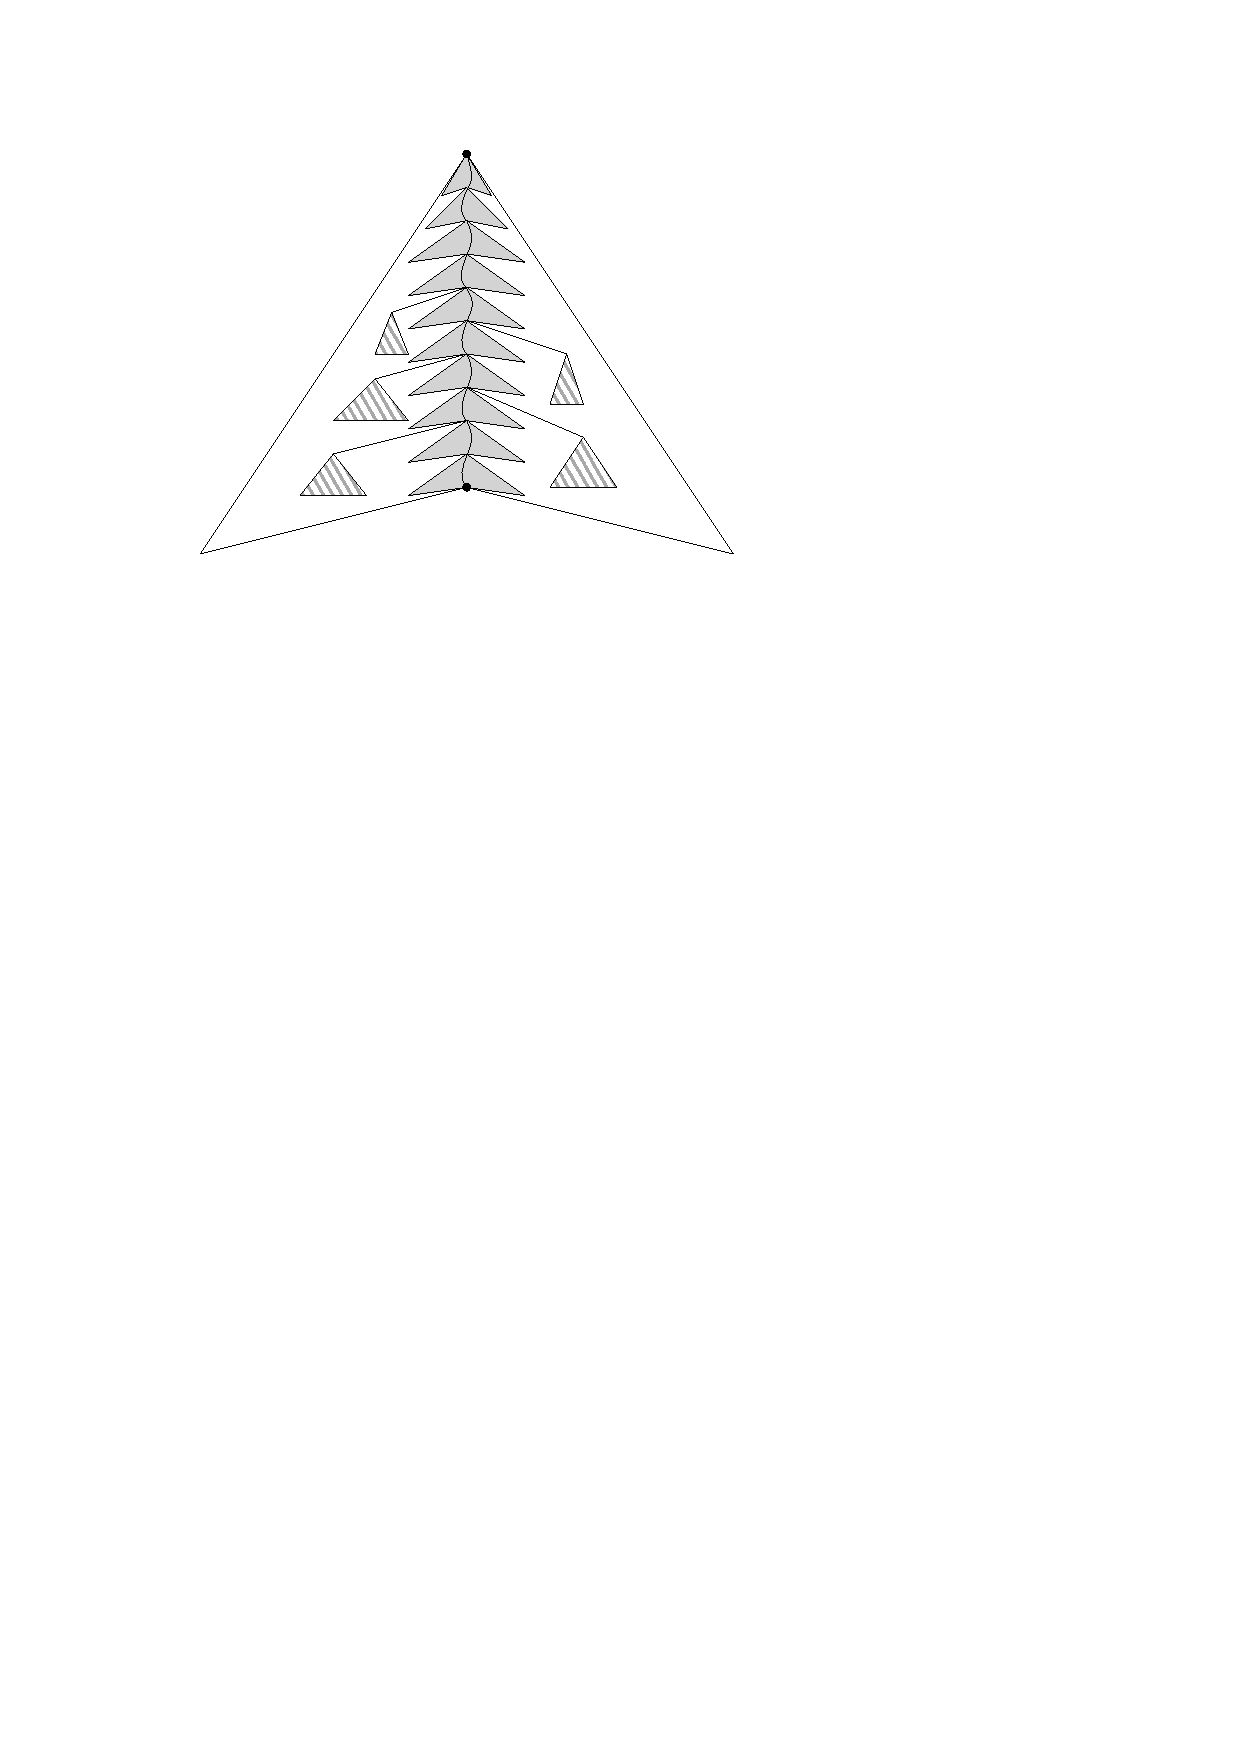
\includegraphics[scale=1]{refinement}
\end{center}
\caption{A large fragment containing a number of smaller fragments. The small fragments on the spine are gray, and the subtrees hanging off of the spine are black (each of them may contain many small fragments). %We start by reducing the hanging subtrees to just two nodes, then handle the small active fragments on the spine, and finally reduce the entire large fragment to one caterpillar and process it. 
\label{figure of small fragments inside a large fragment}}
\end{figure}


\noindent In Subsection~\ref{section:lemma1} we show how to reduce the hanging subtrees to at most two nodes, one candidate and one certain. Then, in Subsection~\ref{section:lemma2} we reduce the small active fragments on the spine to caterpillars. This turns the entire fragment into a large caterpillar. In Subsection~\ref{section:lemma3} we prune this large caterpillar so that it becomes monotone and without collisions. Finally, in Subsection~\ref{section:lemma4} we preprocess the resulting large caterpillar for eliminated suffix queries. 

\subsection{Partitioning into fragments}\label{section:partioioning}
Our partitioning is obtained by repeatedly applying the following lemma. Let $\alpha$ be the constant hidden in the statement of Lemma~\ref{basic partitioning lemma}.

\begin{lemma}\label{good partition refinement lemma}
Given a good partition of a binary tree into $n/b^{4}$ fragments each of size at most $\alpha^{\ell}\cdot b^{4}$, there
exists a good partition of the tree into $n/(2^b)^{4}$ fragments each of size at most $\alpha^{\ell+1}\cdot (2^{b})^{4}$,
where every fragment in the first partition is contained inside a fragment in the second partition.
\end{lemma}
\begin{proof}
Define $T'$ as the tree obtained by collapsing each fragment of the given partition into a single node. Apply 
Lemma \ref{basic partitioning lemma} to $T'$, with the parameter set to $B= {(2^{b})^{4}}/{b^{4}}$. We obtain
$\frac{n/b^4}{B}=n/(2^{b})^{4}$ fragments. Each of them corresponds to a fragment of the original tree of size at
most $\alpha\cdot \alpha^{\ell}\cdot b^{4}\cdot B = \alpha^{\ell+1}\cdot (2^{b})^{4}$.
\end{proof}

\noindent The entire partition is obtained by applying Lemma~\ref{good partition refinement lemma} $\log^{*}n$ times. 
If $b_{\ell}$ denotes the value of the parameter $b$ in the $\ell$-th application, then  $b_{\ell+1}=2^{b_{\ell}}$. The time to construct the $(\ell+1)$-th partition is $O(n/(b_{\ell})^{4})=O(n/b_{\ell})$. The overall time to construct all partitions is therefore 
$$ O(\sum_{\ell} {n}/{b_{\ell}}) = O(\sum_{\ell} {n}/{2^{\ell}}) = O(n).$$
Observe that the size of a (large) fragment in the $(\ell+1)$-th partition is at most $\alpha^{\ell+1} \cdot (b_{\ell+1})^{4}$ which is at most $O((b_{\ell+1})^5)$ for a large enough $\ell$.\footnote{For sufficiently large $\ell$ we have that $\alpha^{\ell+1}\leq 2^{2^{\ell+1}}$ and $b_{\ell+1}\geq 2^{2^{\ell+1}}$.}  Denoting by $b=b_{\ell}$ and $B=b_{\ell+1}$  we get that every large fragment is of size $O(B^5)$ and is composed of (small) fragments of the $\ell$-th partition (each of size $O(b^5)$). 








\subsection{Reducing a hanging subtree into two nodes}\label{section:lemma1}
The first step in reducing a large fragment into a caterpillar is reducing the hanging subtrees of the large fragment into at most two nodes. The following lemma shows that this can be done in total $O(n)$ time for all fragments in all the $\log^* n$ partitions.




\begin{lemma}\label{lemma1}
	The hanging subtrees of the large fragments in all the partitions can be reduced to at most two nodes (one candidate and one certain) in total $O(n)$ time. 
\end{lemma}
\begin{proof}
We 
perform a heavy path decomposition on each hanging subtree. Since each such subtree is contained in a large fragment, its 
size is bounded by $O(B^5)$, and so we have at most $O(\log B)$ levels in the heavy 
path decompositions. On each level we run Frederickson's search (similarly to what we have presented before).
We run this search in parallel, for all heavy paths from all these hanging subtrees in all large fragments.
The number of  nodes in each level for all the heavy paths together is at most $m=n$ and we set
the parameter $p$ (in Theorem~\ref{Frederickson's theorem}) to $\frac{n}{B^{10}}$, so the number of calls to the $(\frac{n}{b^4} \cdot \log b)$ time feasibility test
is $O(\max \lbrace \log(\max_{j} \lbrace n_j \rbrace), \log(\frac{m}{p+1}) \rbrace) = O(\max \lbrace \log (B^{5}), \log(\frac{n}{n/B^{10}} \rbrace) = O(\log B)$ per level, so
$O(\frac{n}{b^4} \cdot \log b \cdot \log^{2} B) = O(\frac{n}{b})$ for every iteration.
Summing over all $\log^{*}n$ iterations, this is $O(\sum_{\ell}\frac{n}{b_\ell}) = O(n)$.

Constructing the heavy path decompositions and then running Frederickson's search takes linear time in the number
of nodes in the subtrees. If all of them were then reduced to at most two nodes, one candidate and one certain
node for each subtree, this would take $O(n)$ time when summed over all the $\log^{*}n$  iterations. However, we have set
the parameter $p$ to $\frac{n}{B^{10}}$. Thus, considering all the levels, there
might be up to $\log B\cdot\frac{n}{B^{10}}\leq \frac{n}{B^{9}}$ large fragments in which we cannot fully reduce
all the hanging subtrees. These are the active large fragments. We preprocess such fragments naively in time linear in their size. 
This requires only $O(\frac{n}{B^{4}})$ per iteration (and so $O(n)$ overall) since the total size of all active large fragments is at most
$\frac{n}{B^9} \cdot O(B^5)$. 
%We cannot amortize the time spent on processing their hanging
%subtrees  by simply saying that each such hanging subtree is reduced to at most
%two nodes, but we can easily afford to separately pay $O(\frac{n}{B^{4}})$ per iteration for this processing.
\end{proof}


\subsection{Reducing a small active fragment into a caterpillar}\label{section:lemma2}
Having processed the hanging subtrees, we now deal with the active small fragments on the spine of the large fragment. 

\begin{lemma}\label{lemma2}
	The small active fragments on the spines of all large fragments can be reduced to caterpillars in total $O(n)$ time. 
\end{lemma}
\begin{proof}

In the previous iteration we had $O(\frac{n}{b^9})$ active fragments, which is of course
too many for the current level. We take the remaining active small fragments (the ones on spines of large 
fragments), and reduce them to caterpillars (again by constructing the heavy path decomposition and running
Frederickson's search with $p$ set to $\frac{n}{B^{10}}$). In each fragment we have $O(\log b)$ levels of the heavy
path decomposition, and for each level we need $O(\log B)$ calls to the feasibility test, which takes
$O(\frac{n}{b^4} \cdot \log b \cdot \log B \cdot \log b) = O(\frac{n}{b})$ time in total. We also do linear
work exclusive of feasibility tests. This processing of small active fragments takes $O(n)$ time over all
$\log ^*n$ iterations, by the same reasoning as for the hanging subtrees.
\end{proof}


We now have $O(\frac{n}{B^9})$ small active fragments in total. We declare each large fragment that contains a small active fragment as active. 

\subsection{Pruning the resulting large caterpillar}\label{section:lemma3}
So far, each inactive large fragment was reduced to one large caterpillar consisting of the concatenation of caterpillars from the smaller fragments on its spine. We want
to prune this large caterpillar (as we have done to the inactive fragments before) in order to ensure
that it is monotone and contains no collisions.   Then, we will
be able to preprocess the caterpillar for every possible eliminated suffix.

\begin{lemma}\label{lemma3}
	The inactive large fragments can be processed in overall $O(n)$ time so that each of them is a caterpillar, the distances of the leaves from the root and the hole are monotone, and there are no collisions between candidate nodes and certain nodes.
\end{lemma}
\begin{proof}

We start by pruning the large caterpillar so that distances of the candidates from the root are
monotone. Since the distances are monotone inside each small caterpillar, we only have to check the last (bottom most) 
candidate node of a small caterpillar against a range of consecutive candidates nodes below it in the large
caterpillar, starting from the top candidate node in the next small caterpillar. 
At this point we need to be more precise about how the fragments are represented. Each inactive small
fragment has been reduced to a caterpillar. For each such caterpillar, we maintain a doubly-linked list containing
all of its candidate nodes in the natural order, and additionally we store the first and the last certain
node (nearest to the root and to the hole, respectively). Assuming such representation, we traverse
the large caterpillar from bottom to top while
maintaining a stack with the already processed small caterpillars that still contain some candidate nodes.
We retrieve the last candidate of the current small caterpillar and eliminate the appropriate candidate
nodes below it. This is done by iteratively retrieving the top small caterpillar from the stack and then
accessing its top remaining candidate node $u$. If the distance of $u$ from the root is too small, we
remove $u$ from the front of its doubly-linked list, pop the list from the stack if it becomes empty,
and repeat. Now the distances of the remaining candidates from the root are
non-decreasing. We repeat the symmetric process from top to bottom to ensure that also the distances
from the hole are non-decreasing. The whole procedure takes linear time in the number of eliminated
candidate nodes plus the number of small fragments, which sums up to $O(n)$ overall.

Now we need to eliminate all internal ``collisions'' inside the large caterpillar (i.e. remove candidate nodes that
are too close to certain nodes). These collisions can occur between a candidate node of one small caterpillar
and a certain node of another small caterpillar. Each certain node eliminates a range of consecutive
candidates nodes below and above its small caterpillar. Therefore, we only need to consider the 
last certain node of a small caterpillar and a range of consecutive candidate nodes below it in the
large caterpillar, starting from the top candidate node in the next caterpillar (and then repeat
the reasoning for the first certain node and a range of candidates nodes above it). This seems very similar
to the previous step, but in fact is more complex: a certain node $v$ eliminates a candidate node $u$ when
$d(u,v)<\lambda^{*}$, but we do not know the exact value $\lambda^{*}$ yet! Therefore, we need to run
a feasibility test to determine if $u$ should be eliminated. We cannot afford to run many such tests
independently and hence will again resort to Frederickson's search. Before we proceed, observe that
it is enough to find, for every small caterpillar, the nearest certain node $v$ above it, and then determine
the prefix of the small caterpillar that is eliminated by $v$. To find $v$ for every small caterpillar,
we first traverse the large caterpillar from top to bottom while maintaining the nearest certain node
in the already seen prefix.

To apply Frederickson's search, we would like to create a matrix of dimension $1\times O(b^{5})$
for each of the $O(\frac{n}{b^{4}})$ small caterpillars in the whole tree. The total size of all small
caterpillars is at most $m=n$, so setting $p$ to $\frac{n}{B^9}$ would imply
$O(\max \lbrace \log(\max_{j} \lbrace n_j \rbrace), \log(\frac{m}{p+1}) \rbrace) = O(\max \lbrace \log (b^{5}), \log(\frac{n}{n/B^{9}} \rbrace) = O(\log B)$ calls to the $O(\frac{n}{b^{4}} \cdot \log b)$ time test.
There are two difficulties, though. First, we cannot guarantee that the processing exclusive of feasibility tests
would sum up to $O(n)$ over all iterations. Second, it is not clear how to provide constant time access
to these matrices, as the candidates nodes inside every small caterpillar are stored in a doubly-linked list,
so we are not able to retrieve any of them in constant time. 
%We could have maintained the candidate
%nodes in an array, but then after the whole pruning and eliminating we would need to merge the arrays
%of all small caterpillars to obtain the array of the large caterpillar, which  does not seem possible
%in constant time (and we cannot afford to spend much more per a small caterpillar).

We mitigate both difficulties with the same trick. We proceed in $O(\log b)$ steps that, intuitively, correspond
to binary searching for how long should the eliminated prefix be. In the $i$-th step we
create a matrix of dimension $1\times 2^{i}$ for each of the still remaining small caterpillars.
The matrix is stored explicitly, that is we extract the top $2^{i}$ candidates nodes from the doubly-linked
list and store them in an array. We set $p$ to $\frac{n}{B^{10}}$ and run Frederickson's search
on these matrices. The total time for all feasibility tests is then
$O(\frac{n}{b^{4}}\cdot \log b \cdot \log b \cdot \log b) = O(\frac{n}{b})$. 
Then, if all $2^{i}$ candidate nodes have been eliminated, we proceed to the next
step. Otherwise we have already determined the small caterpillar's prefix that should be eliminated.
Observe that the total length of all arrays constructed during this procedure is bounded by the number
of eliminated candidate nodes multiplied by 4. Consequently, both the time necessary
to extract the top candidate nodes (and arrange them in an array) and the time exclusive of feasibility tests sums up to $O(n)$
over all iterations. During this process we might declare another $O(\frac{n}{B^9})$ large fragments active
by the choice of $p$.
\end{proof}


\subsection{Preprocessing the large caterpillar for every possible eliminated suffix}\label{section:lemma4}

Having reduced a large fragment to a large caterpillar, we are now left only with preprocessing this large caterpillar for every possible eliminated suffix.
Because we have already pruned the large caterpillar and removed any collisions between a certain
node and a candidate node, we only have to consider the remaining candidate nodes.
Recall that in the previous algorithm we stored at the bottom node of every prefix of the caterpillar
the following information: the number of chosen nodes, the candidate node, and the certain node for this fragment,
assuming that the suffix below this node is eliminated. Now however, we cannot afford to explicitly
compute such information for every node in every iteration,
as this might take linear time per iteration. We start with reinterpreting it in terms of
\emph{jump pointers}. 

\paragraph{Jump pointers.} For each candidate node in a caterpillar, its jump pointers leads to the nearest
candidate above (in the same caterpillar) that is at distance at least $\lambda^{*}$. Then, the information
stored at the bottom node $u$ of every prefix can be computed by starting at $u$ and following
the jump pointers as long as possible. The number of nodes chosen for the solution is simply the number of visited
nodes. If the last visited node is at distance at least $\frac{\lambda^{*}}{2}$ from the root then it is
the certain node, and otherwise the last visited node is the candidate node and its predecessor
(if any) is the candidate node. We would like to maintain such information for all nodes $u$,
such that $u$ might be accessed in query time. Recall that in query time we specify
a node $v$ attached to the hole of the fragment and binary search for the first node $u$ that
is at distance at least $\lambda^{*}$ from $v$. Therefore, we only need to maintain the information
for a suffix consisting of nodes that are not too far from the hole (i.e. at distance at most $\lambda^{*}$). However, it is not
 trivial to update such information after merging multiple small caterpillars into
one. This is because we might remove some nodes (a prefix and a suffix)
from every small caterpillar before the merge. To overcome this, we divide every caterpillar into
three parts as described below.

\paragraph{The unstable prefix,  unstable  suffix, and stable infix.} 


Consider a caterpillar with root $r$ and hole $h$, and let $u_{i}$ denote its $i$-th candidate node. In Lemma~\ref{lemma3} we have already made sure that $d(r,u_{i}) < d(r,u_{i+1})$
and that $d(h,u_{i}) > d(h,u_{i+1})$. We define the \emph{unstable prefix} to
consist of all nodes $u_{i}$ such that $d(r,u_{i})\leq \frac{\lambda^{*}}{2}$, and similarly the
\emph{unstable suffix} consists of all nodes $u_{i}$ such that $d(h,u_{i})\leq \frac{\lambda^{*}}{2}$.
The remaining nodes $u_{i}$ are called the \emph{stable infix}.  We have the following property.

\begin{lemma}
\label{stable infix}
If a node of a small caterpillar is removed due to the pruning or collision elimination then it
belongs to the unstable prefix or to the unstable suffix.
\end{lemma}

\begin{proof}
Because of symmetry, it is enough to consider a small caterpillar and all the subsequent
small caterpillars. If a candidate node $u_{i}$ of the former is pruned then there is a top candidate node
$v$ of one of the subsequent caterpillars such that $d(h,u_{i}) < d(h,v)$, where $h$ is the hole
of the large caterpillar. But the distance of $v$ from the spine is less than $\frac{\lambda^{*}}{2}$ (since it is a candidate node),
 and it follows that the distance of $u_{i}$ to the hole of its small caterpillar is also less
than $\frac{\lambda^{*}}{2}$. If $u_{i}$ collides with a certain node $v$ of one of the subsequent
caterpillars then $d(u_{i},v)<\lambda^{*}$. But the distance of $v$ from the spine is at least
$\frac{\lambda^{*}}{2}$, so the distance of $u_{i}$ to the hole of its small caterpillar must be
less than $\frac{\lambda^{*}}{2}$. Hence, $u_{i}$ belongs to the unstable suffix.
\end{proof}

We maintain the unstable prefix and the unstable suffix  in a balanced search
tree (sorted by the distance to the root) that allows split and merge in logarithmic time.
The stable infix is maintained in a separate structure that allows us to efficiently simulate traversing jump pointers inside the stable infix. 
%
In query time, we first use the balanced search tree storing the unstable suffix to locate the bottom-most node
$u_{i}$ that is sufficiently far away. Observe that after taking $u_{i}$ we cannot
take any further nodes from the unstable suffix, as they are all within distance less than
$\lambda^{*}$ from each other. Hence, we need to continue in the stable infix (it can also
happen than no $u_{i}$ from the unstable suffix can be taken, and we directly start in the stable
infix). Then, we use the structure maintained for the stable infix, which gives us the top-most
node that we would reach by following up the jump pointers. Finally, we  continue in the unstable prefix. 

By the same argument as before, we can visit at most one node in the unstable prefix.
Therefore, if we can efficiently answer a query in the stable infix, then answering a query in
the whole caterpillar requires only additional logarithmic time (in the size of the caterpillar).
Additionally, after merging multiple small caterpillars into one, we need to determine the unstable
prefix and the unstable suffix of the resulting large caterpillar and make sure that we have
their corresponding binary search trees available.
Then we have to construct the structure for the stable infix of the large caterpillar.
We next describe these two steps.

\paragraph{Maintaining the unstable suffixes.}
Consider the unstable suffix of the large caterpillar (the situation for the unstable prefix is
symmetric). It is easy to see that all of its nodes are contained in unstable suffixes of
the small caterpillars. We merge all the binary search trees storing these unstable suffixes.
This takes $O(\log (B^5))$ time per merge, so $O(\frac{n}{b^{4}}\cdot \log (B^5))=O(\frac{n}{b})$ in total.
Then, we binary search to determine how many nodes are actually sufficiently close to the hole of the large caterpillar, and
 split the binary search tree accordingly in $O(\log (B^{5}))$ time. To implement binary search, we need to
check if a distance from a node to the hole is at least $\frac{\lambda^{*}}{2}$, but of course we
do not know $\lambda^{*}$ yet. Therefore, we perform all these binary searches in parallel. We proceed in $O(\log (B^{5}))$ rounds. In every round we apply Frederickson's search
with parameter $p$ set to $\frac{n}{B^{10}}$ to determine  the outcome of the comparison for all
but $\frac{n}{B^{10}}$ binary searches. This needs
$O(\frac{n}{b^{4}}\cdot\log b\cdot\log B\cdot\log B)=O(\frac{n}{b})$ additional time for
all the feasibility tests and creates additional $O(\frac{n}{B^{9}})$ active large fragments.

\paragraph{Maintaining the stable infixes.}
We now describe the structure for maintaining the stable infix of a caterpillar consisting of candidate nodes $u_{1},u_{2},\ldots,u_{k}$ with root $r$ and hole $h$. 
Recall that, for each candidate node $u_i$, its jump pointers lead to the closest candidate node above it (in the same caterpillar) that is at distance at least $\lambda ^*$. 
We need a structure that allows us to query, given a node $u$ attached to $h$, for the nearest candidate node $u_{i}$ at distance at least $\lambda^{*}$ from $u$, and then follow the jump pointers from $u_{i}$.
%
Observe that we only consider $u$ such that $d(r,u)\geq d(r,u_{k})$. This is because either $u$ is a certain node and then its distance from the hole is at least
$\frac{\lambda^{*}}{2}$, or $u$ is a subsequent candidate node from the same caterpillar,
or we start the query with comparing these two distances.

We are interested in the number of traversed jump pointers and in the last visited node.
%(because of the unstable prefix, we do not need to retrieve both the last node
%and its predecessor). 
During the preprocessing, we need to merge multiple stable infixes
into one, while possibly inserting some nodes in-between (these new nodes have previously
belonged to some unstable prefixes and suffixes). To find $u_{i}$, we keep all candidate
nodes of a caterpillar in a mergeable balanced search tree. This allows us to locate $u_{i}$
in logarithmic time (in the size of the caterpillar), and the total time to construct the balanced
search trees for all stable infixes by merging the smaller balanced search trees
is $O(\frac{n}{b^{4}}\cdot \log (B^{5}))=O(\frac{n}{b})$. Note that the smaller balanced search
trees could either be associated with a stable infix of a small caterpillar or be obtained
by splitting a balanced search tree stored for an unstable prefix or an unstable suffix of
a small caterpillar.
We will show how to maintain the answer, that is the number of traversed jump pointers and the
last visited node, explicitly for every $u_{i}$ that could be queried.

We write $\jump(i)=j$ if the jump pointer of $u_{i}$ points to $u_{j}$, where $j<i$, and $\jump(i)=-1$
if the jump pointer of $u_{i}$ is not defined, that is $d(u_{1},u_{i})<\lambda^{*}$.
The {\em interesting prefix} of the caterpillar consists of all nodes $u_{i}$ such that $\jump(i)=-1$,
and the {\em interesting suffix} consists of the nodes $u_{\jump(k)},u_{\jump(k+1)},\ldots,u_{k}$.
Because we always query with a node $u$ such that $d(r,u) \geq d(r,u_{k})$, we only
need to maintain the answer for the nodes in the interesting suffix. As a special case,
if $\jump(k)=-1$ we call the caterpillar \emph{fresh}.
After merging multiple small caterpillars into one we might need to update some of the jump pointers.
However, once a jump pointer has been set, it will never change. Therefore, we might only
need to set up the jump pointers in the interesting prefixes of the small caterpillars
(and the new nodes inserted in-between). We also observe that these new jump pointers
must lead either to a node in the interesting suffix of some small caterpillar
or to some new node. We start with checking if the large caterpillar is fresh. This can be
done by applying Frederickson's search in parallel for all large caterpillars with $p$ set to
be $\frac{n}{B^{9}}$, using $O(\frac{n}{b^{4}}\cdot \log b \cdot \log B)=O(\frac{n}{b})$
total time for the feasibility tests and creating up to $O(\frac{n}{B^{9}})$ additional active large
fragments. If a large caterpillar is fresh, there is nothing to update. Otherwise,
we gather all candidate nodes belonging to
an interesting prefix or suffix (or being a new node) and call them \emph{relevant}. In particular,
all nodes of a fresh small caterpillar are relevant.
We arrange all relevant nodes in an array and apply Frederickson's search to determine the missing jump
pointers using the array to facilitate constant time access to any relevant node. We again
set $p$ to be $\frac{n}{B^{9}}$, need $O(\frac{n}{b^{4}}\cdot \log b \cdot \log B)=O(\frac{n}{b})$
time for the feasibility tests, and create $O(\frac{n}{B^{9}})$ additional active large fragments.
The time exclusive of the feasibility tests is bounded by the number of relevant nodes.
We claim that once we know all the missing jump pointers we can actually update the answers
for all nodes in the interesting suffix of the large caterpillar in time proportional to the
number of relevant nodes. This is because all nodes of that interesting suffix are
relevant, and we can update the answer for all relevant nodes by traversing them from top
to bottom. The current candidate node either already had a jump pointer before, and hence
we can use its previously computed answer to access an already processed relevant node
(as all nodes in an interesting prefix are relevant, and the answer is always a node in an
interesting prefix by definition) and, by combining with the already updated answer for that
relevant node, recalculate the answer, or follow its freshly found jump pointer to also access
an already processed relevant node. The total time for this update is again proportional to the
number of relevant nodes. It remains to bound this quantity. We claim that it
amortizes to $O(n)$. To this end, we maintain the following invariant: every node
of an interesting prefix and suffix has one credit. If a caterpillar is fresh
then every node $u_{1},u_{2},\ldots,u_{k}$ has two credits. Initially, every node of the tree
has two credits. When a node becomes a part of a stable infix we treat it as a small fresh
caterpillar in the analysis. The number of relevant nodes is bounded by the total number
of nodes in all fresh small caterpillars and the total number of nodes in the interesting
prefixes and suffixes in the remaining small caterpillars. Furthermore,
the interesting prefix (and similarly the interesting suffix) of the resulting large caterpillar
consists of nodes belonging to fresh small caterpillars and the interesting prefix of
some small caterpillar. So to pay for all relevant nodes and then make sure that the invariant
still holds we only need additional $O(b^{5})$ credits (to pay for the interesting prefix
of some small caterpillar and the interesting suffix of some small caterpillar) per large
caterpillar. This sums up to $O(\frac{n}{B^{4}}\cdot b^{5}) = O(\frac{n}{b})$ per iteration.

To conclude, we have shown how to obtain an $O(\frac{n}{B^{4}}\log B)$ time test given an $O(\frac{n}{b^{4}}\log b)$
time test. The preprocessing time is $O(\frac{n}{b})$ per iteration plus amortized constant per
node of the tree. After $\log ^*n$ iterations, we have a $O(\frac{n}{\log ^4n} \cdot \log \log n)$ test,
which we use to solve the dispersion optimization problem in linear time. All iterations of the preprocessing
cost $O(n)$ time altogether.
% why do we stop at fragments of size polylog(n)? Can't we get one large fragment?


\section{The Weighted Dispersion Problem}
We now consider the weighted variant of the dispersion problem, in which not only the edges have weights, but also the nodes. Recall that $f(P)=\min_{u,v\in P} \{d(u,v)\}$. The weighted problems are defined as follows.
\begin{itemize} 
\item {\em The Weighted Dispersion Optimization Problem.} Given a tree with non-negative edge lengths, non-negative node weights, and a number $W$, find a subset of nodes $P$ of weight at least $W$, such that  $f(P)$ is maximized. 

\item {\em The Weighted Dispersion Decision Problem.} Given a tree with non-negative edge lengths, non-negative node weights, a number $W$, and a number $\lambda$, find a subset of nodes  $P$ of weight at least $W$, such that $f(P)\geq\lambda$. 
\end{itemize}


In this section we present an $O(n\log n)$ time algorithm (feasibility test) for the weighted decision problem, and prove that it is optimal, by giving an $\Omega(n\log n)$ lower bound in the algebraic computation tree model. We then present an $O(n\log^2 n)$ time algorithm for the weighted optimization problem. 

\subsection{An \boldmath$ \Omega (n\log n)$ lower bound for the weighted feasibility test}

In the {\em Set Disjointness Problem}, we are given two sets of real numbers $X=\lbrace x_1,x_2,...,x_n \rbrace$ and $Y=\lbrace y_1,y_2,...,y_n \rbrace$ and we need to return true iff $X \cap Y = \emptyset$. 
It is known that solving the set disjointness problem requires $\Omega(n \log n)$ operations in the algebraic
computation tree model~\cite{BenOr}. %, where $|X|=|Y|=n$. % (this subsumes the well-known lower bound in the decision tree
%model).
We present a reduction from the set disjointness problem to the weighted feasibility test problem. We assume without loss of generality that the elements of $X$ and $Y$ are non-negative~\footnote{Otherwise
we can simply find the minimum element, and subtract the minimum from all the elements.}.


Given the two sets $X$ and $Y$, we construct a tree $T$ as follows. We first compute and set
$K := 2 \cdot \max (X\cup Y) +3$.
The tree $T$ contains two vertices of weight zero, $u$ and $v$, that are connected by an edge of length $\frac{K}{2}$. In addition, for each element $x_i \in X$, we have a node of weight $x_i+1$, that is connected to $u$ by an edge of length $\frac{K}{2} - x_i -1$. For each element $y_i \in Y$, we have a node of weight $K - y_i -1$, that is connected to $v$ by an edge of length $y_i+1$.
\begin{lemma}
$X \cap Y = \emptyset$ iff the weighted feasibility test returns false for $T$ with  parameters $W=K$ and $\lambda =K$.
\end{lemma}

\begin{proof}
We start by proving that if $X \cap Y \neq \emptyset$ then there is a subset of the vertices of the tree, $P \subseteq T$, s.t. $W(P) \geq K$ and $f(P) \geq K$ (where $W(P)$ is the sum of the weights of all the vertices in $P$). Suppose that  $x_i=y_j$. Then, $d(x_i,y_j) = d(x_i,u) + d(u,v) + d(v,y_j) = \frac{K}{2} - x_i -1 + \frac{K}{2} + y_j +1 = K \geq K$. Furthermore, $W(x_i) + W(y_j) = x_i + 1 + K- y_j -1 = K \geq K$, and so the feasibility test should return true with $P = \lbrace x_i, y_j \rbrace$.

Now we need to prove that if the feasibility test returns true, the sets are not disjoint.
We start by proving that any feasible subset $P$ cannot have more than one vertex from each of the sets.
Assume for contradiction that $P'$ is a feasible subset that contains at least two vertices that correspond to elements of $X$. Denote these two vertices by $x_i$ and $x_j$. We assume that $P'$ is a feasible solution, and so $d(x_i,x_j) \geq K$. But, $d(x_i,x_j) = \frac{K}{2} - x_i -1 + \frac{K}{2} - x_j -1 = K - x_i - x_j -2 < K$ (since $x_i$ and $x_j$ are non-negative) and we have a contradiction.
The second case (when $P'$ contains two elements of $Y$) is symmetric. %We assume for contradiction that $Y'$ is a feasible subset that contains at least two vertices that correspond to elements of $Y$. Denote these two vertices by $y_i$ and $y_j$. We assume that $Y'$ is a feasible solution, and so $d(y_i,y_j) \geq K$. But, $d(y_i,y_j) = y_i + 1 + y_j + 1 = y_i + y_j + 2 < K$ and we have a contradiction.
Observe that it is also not possible for $P$ to contain only one node, since the weight of any node is strictly less than $K$. So, we now only need to prove that if $P= \{ x_i,y_j \}$ is a feasible solution, then $x_i = y_j$. We assume that $P= \{ x_i,y_j \}$ is a feasible solution, and so on the one hand $d(x_i,y_j) = \frac{K}{2} - x_i -1 + \frac{K}{2} + y_j +1 = K - x_i + y_j \geq K$ implying that $y_j \geq x_i$. On the other hand, $W(P) = x_i + 1 + K - y_j -1 = K + x_i - y_j \geq K$ implying that $x_i \geq y_j$. We conclude that $x_i = y_j$.
\end{proof}

\subsection{An \boldmath$O(n \log ^2 n)$ Algorithm for the weighted feasibility test}
Similarly to the unweighted case, we would like to compute for each node of the tree, the subset of nodes in its subtree, $P$, s.t. $f(P) \geq \lambda$ and $W(P)$ is maximized. We compute this by going over the nodes of the tree bottom-up. Previously, the situation was simpler, as for any subtree we had just one candidate node that we were not sure would be in the solution for the whole input tree. This was true, because only a node that is closer to the root could be at distance less than $\lambda$ from a certain node, and we could always take the node that is farthest from the root between the two, since nodes were of uniform weight.
Denote by $h$, the node for which $d(h,v)$ is minimized, out of all the chosen nodes in the subtree rooted at $v$. We call $h$ the closest chosen node in $v$'s subtree. For the weighted feasibility test, we will store a solution ($P$) inside the subtree for any possible distance of the closest chosen node in the subtree from its root (up to $\lambda$, since if the closest node is farther, it does not affect nodes outside the subtree). This can be viewed as a monotone polyline, since the weight of $P$ only decreases as the distance of the closest chosen node increases from zero to $\lambda$. The weight of $P$ only changes at certain points, i.e. the breakpoints of the polyline. Each point of the polyline is a key-value pair, where the key is $d(h,v)$, and the value is $W(P)$, the weight of the heaviest possible subset of nodes in the subtree rooted at $v$, s.t. the closest chosen node is at distance greater or equal to $d(h,v)$ from $v$, and for every pair of chosen nodes $x_1,x_2$ it holds that $d(x_1,x_2) \geq \lambda$.

\begin{figure}[h]
\begin{center}
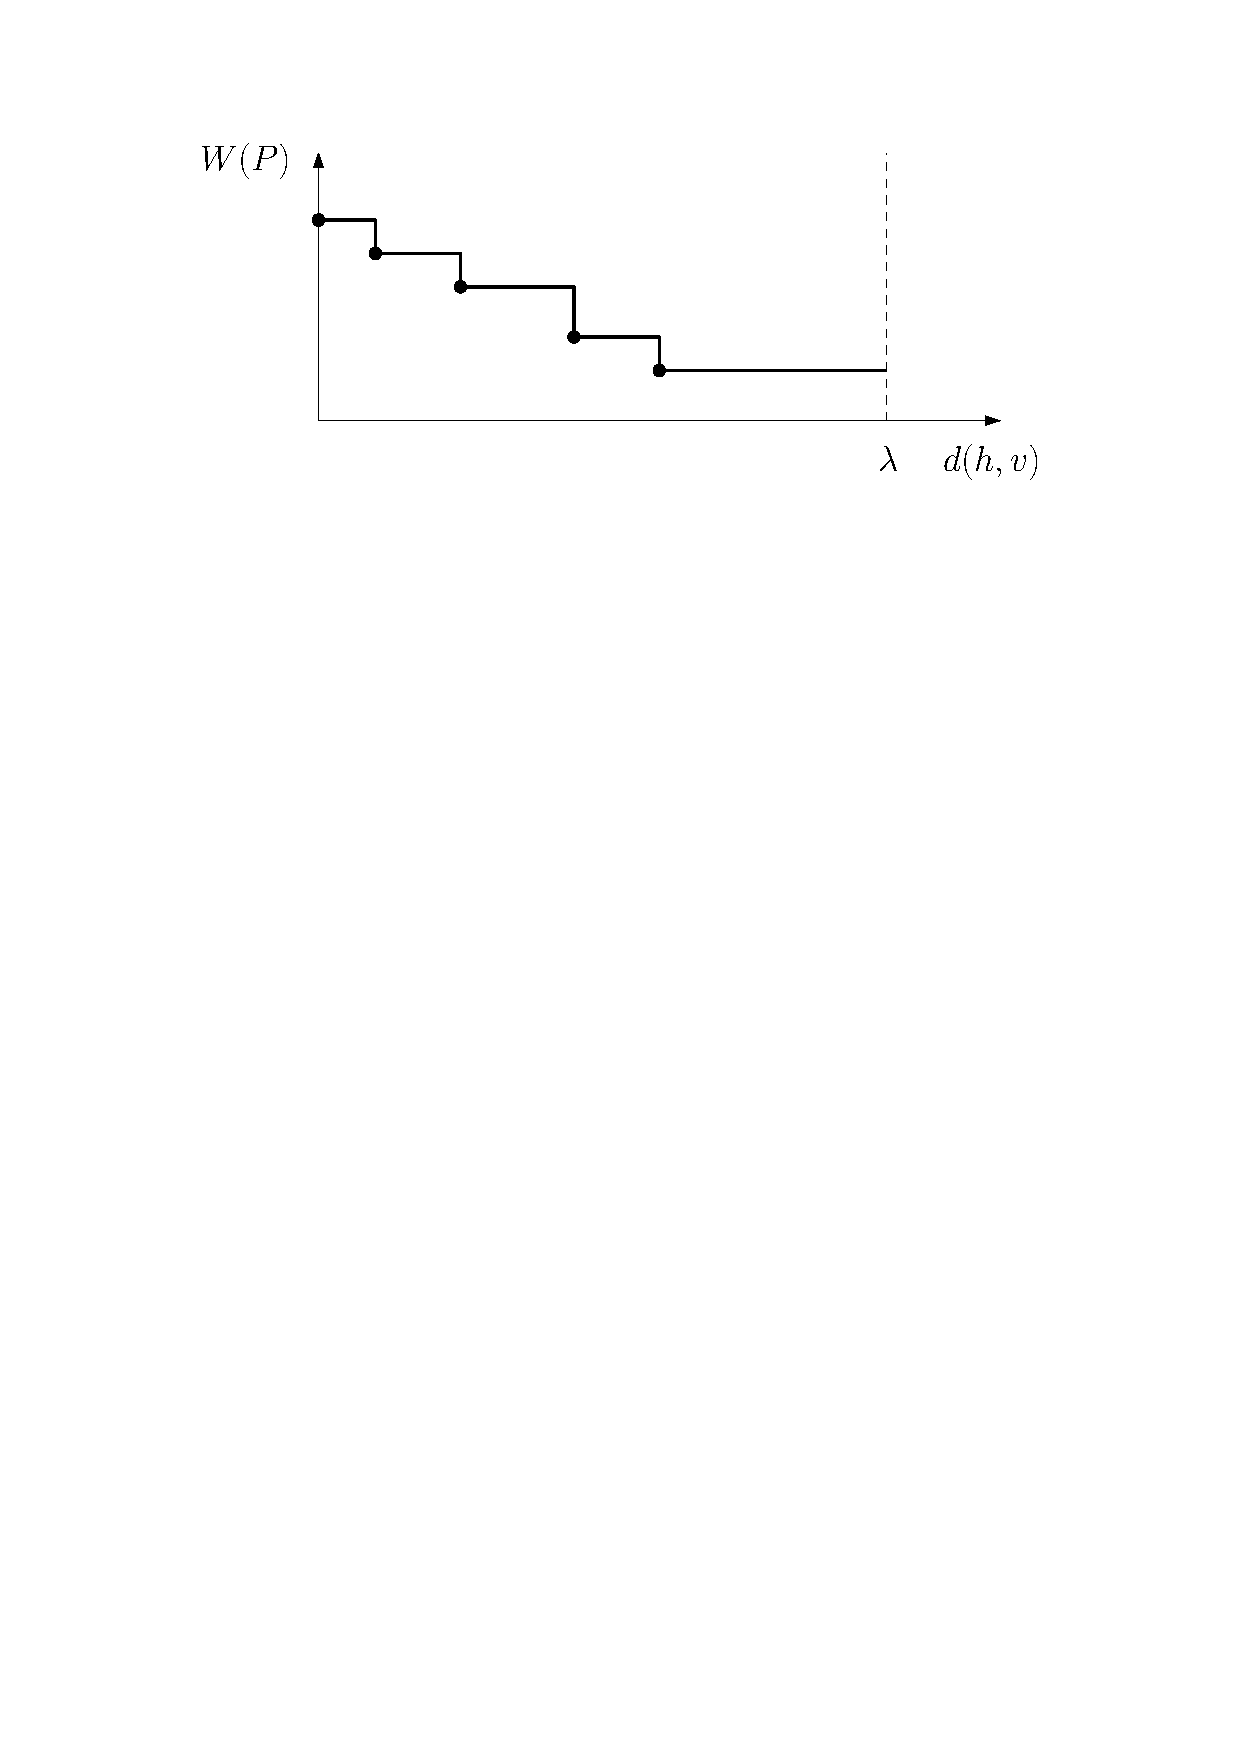
\includegraphics[scale=0.35]{polyline}
\end{center}
\caption{The polyline represents the weight of the solution, $P$, as a function of the distance of the closest chosen node in the subtree. $v$ is the root of the subtree, and $h$ is the chosen node closest to $v$ in its subtree. The weight of $P$ only decreases at certain points, which are the breakpoints of the polyline. The value for a breakpoints itself is the value between it and the next breakpoint.
\label{figure of a polyline}}
\end{figure}

The algorithm we present computes such a polyline for the subtrees rooted at all the nodes of the tree. As we mentioned, we will compute this bottom-up, and so in each step of the algorithm we compute the polyline for a subtree rooted at some node $v$, after we have already computed the polylines for the subtrees rooted at his children. In each step, we wish to use the polylines we have already constructed, and not construct the new polyline from scratch. We achieve this in time $O(x \log y)$, where $x$ is the number of breakpoints in the polyline with fewer breakpoint, and $y$ the number of breakpoints in the other polyline. This sums up to $O(n \log ^2 n)$ overall.

When constructing a polyline, we need to consider several cases, as the closest chosen node in the subtree could be the root, or it could be in the subtree of one of its children. This means that for any key $d(h,v)$ in the polyline, the value for that key can represent a solution $P$ in which $h$ is in the subtree rooted $v$'s left child, or in the subtree rooted $v$'s right child, or it could be $v$ itself.\footnote{For the same reasoning as in the unweighted case, we assume w.l.o.g. that the input tree is binary.}

We now present a single step of the algorithm. We postpone the discussion of the data structure we use to store the polylines for now, and first describe generally how we construct a polyline. Later we state the interface we require of the polylines, and discuss the data structure we use for them and the complexity it induces for the algorithm.

If $v$ only has one child we can simply build the new polyline by querying the previous one for the case that $v$ is in the solution (i.e. query the polyline computed for $v$'s child with distance of the closest chosen node being $\lambda-d(v,v')$, where $v'$ is the child of $v$), and add to this value the weight of $v$ itself. We then construct the polyline by taking the value we got, which will be the value between zero and the first breakpoint, and merging it with the polyline computed for $v'$, shifted right by $d(v,v')$, as we now measure the weight of the solution as a function of the distance of the closest chosen node to $v$, and not $v'$.

If $v$ has two children, denote its left child by $u_1$, and its right child by $u_2$. We have two polylines that represent the solutions inside the subtrees rooted at $u_1$ and $u_2$ (denoted by $p_1$ and $p_2$), and we would like to create the polyline for the subtree rooted at $v$ (denoted by $p$).
Assume w.l.o.g. that the number of breakpoints in $p_1$, is smaller or equal to the number of breakpoints in $p_2$.

Let us consider the case where $v$ is in the solution. In this case we simply query $p_1$ and $p_2$ for their values with distances of the closest node being $\lambda - d(v,u_1)$ and $\lambda - d(v,u_2)$ (if one of these is negative, we take zero instead), add them together with the weight of $v$, and get the weight of the solution for $v$'s subtree in case $v$ is in the solution. This will be the value of the new polyline for $d(h,v)$ between zero and the first breakpoint.

We now construct the rest of the polyline. Notice that we need to maintain that $d(h_1,h_2) \geq \lambda$ (where $h_1$ is the closest chosen node in $u_1$'s subtree and $h_2$ is the closest chosen node in $u_2$'s subtree). First, we need to shift $p_1$ and $p_2$ right by $d(v,u_1)$ and $d(v,u_2)$ respectively (again, because we want to measure the distance of $h$ from $v$, not from $u_1$ or $u_2$). We then proceed in two steps:

\begin{enumerate}
\item We start by constructing the second part of the polyline, where $d(h,v) \geq \frac{\lambda}{2}$. In this case we query both polylines ($p_1$ and $p_2$) with the same key, since $d(h_1,v) \geq \frac{\lambda}{2}$ and $d(h_2,v) \geq \frac{\lambda}{2}$ implies that $d(h_1,h_2) \geq \lambda$. The naive way to proceed, would be to iterate over the second half of both polylines in parallel, and at every point sum the values of the two polylines to get the value of the new polyline. This will not be efficient enough. We would like to be able to not iterate over $p_2$ (the larger polyline). Instead, we go over all the breakpoints of $p_1$ (the smaller of the polylines) where $d(h_1,v)\geq \frac{\lambda}{2}$ (i.e. the second half of the polyline). These breakpoints induce intervals of $p_2$. For each of these intervals we increase the value of $W(P)$ by the value in theses intervals in $p_1$. For this we might need to insert some of the breakpoints from $p_1$ (where there is no breakpoint already in $p_2$). Now the new polyline stores the weight of the solution for the entire subtree of $v$, as we summed up the weight gained in the subtrees rooted at $u_1$ and $u_2$ (for $d(h,v) \geq \frac{\lambda}{2}$). 

\begin{figure}[h]
\begin{center}
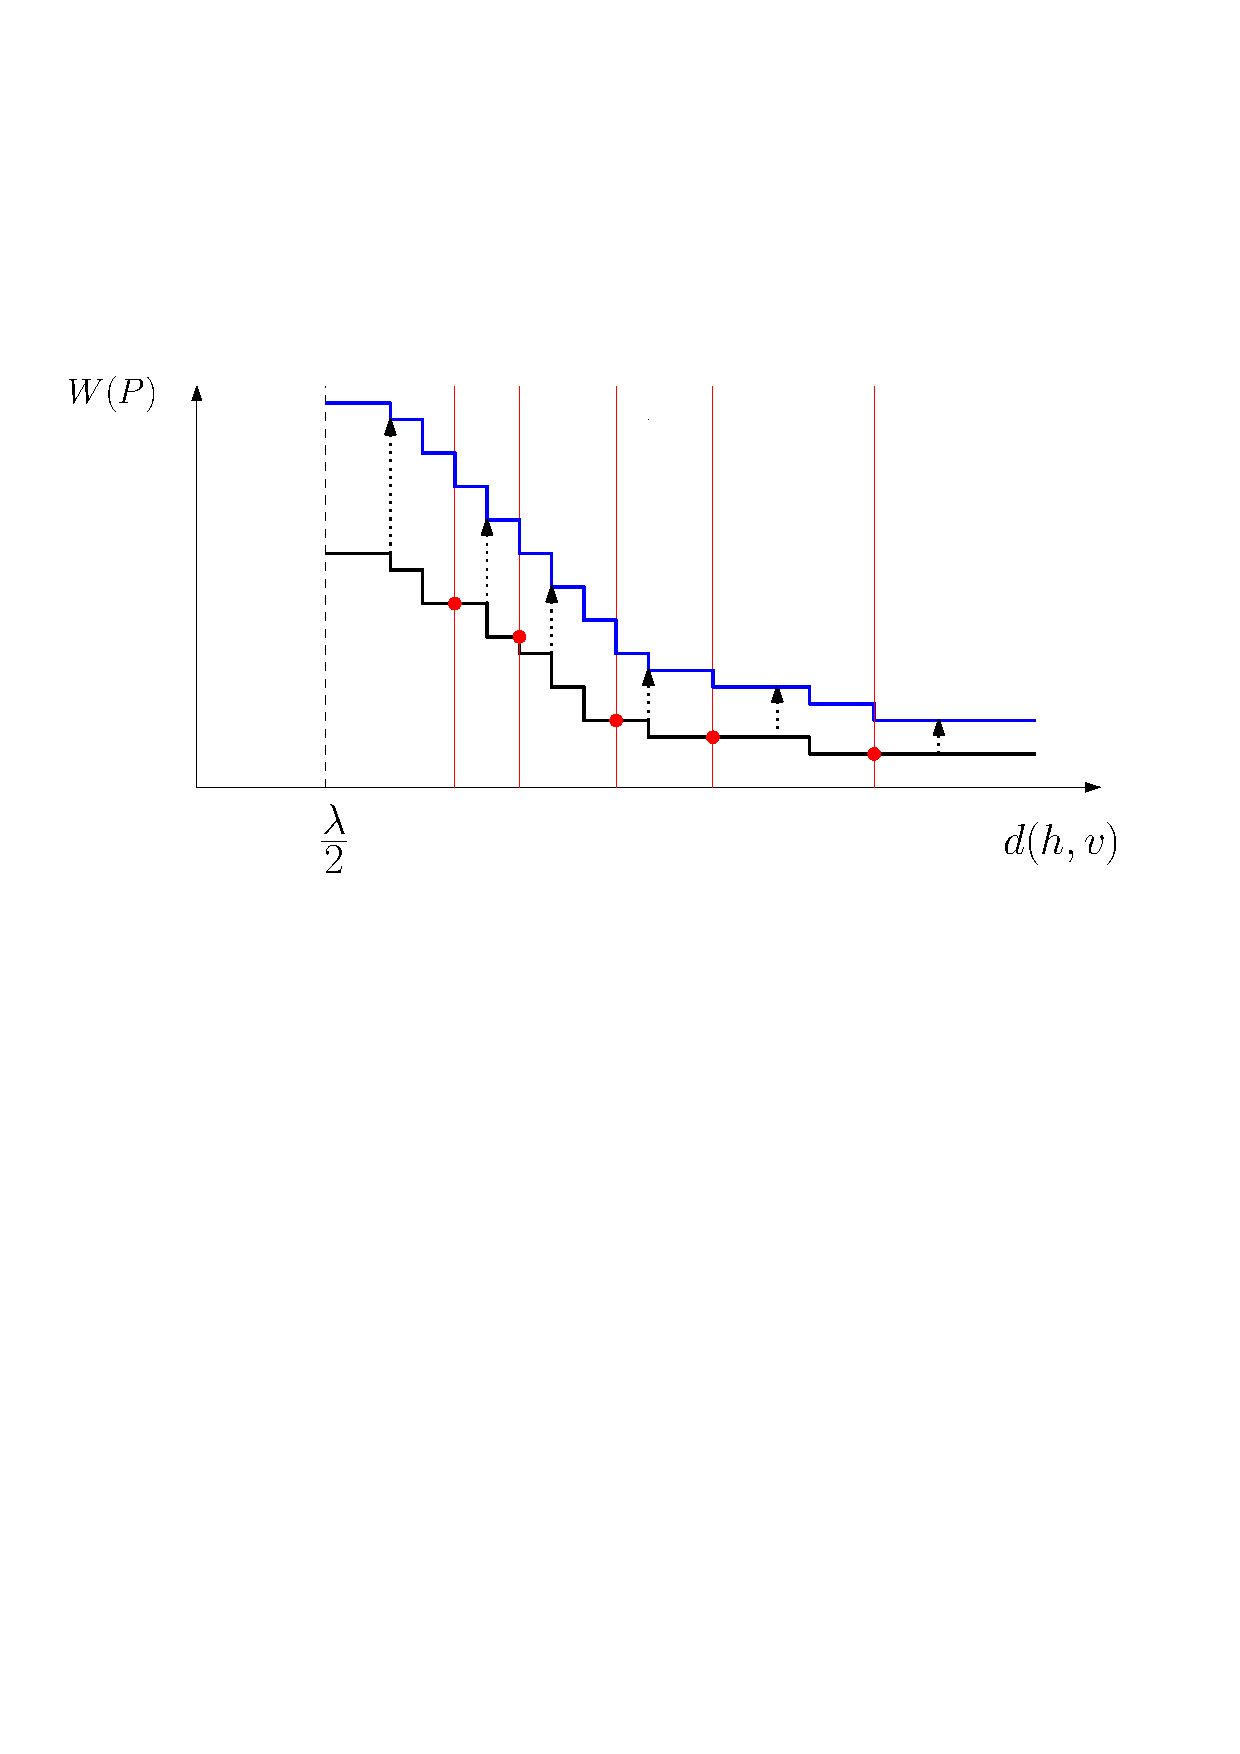
\includegraphics[scale=.5]{new_polyline_second_half}
\end{center}
\caption{Constructing the second half of the polyline. The black polyline is $p_2$. The breakpoints inserted from $p_1$ are in red. In each interval we raise the polyline up by the value in $p_1$ (which is constant, as each interval is between breakpoints of $p_1$).
\label{figure of constructing the second half of the polyline}}
\end{figure}

\item We now need to construct the first half of the polyline, where $d(h,v) < \frac{\lambda}{2}$. For this, we need to consider two possible cases: first, the case where $d(h_1,v) < d(h_2,v)$ (i.e. the closest chosen node in $v$'s subtree is inside $u_1$'s subtree), and second, the case where $d(h_1,v) > d(h_2,v)$. For each of the two cases we will construct the first half of the polyline, and then we take the maximum of the two polylines at every point.

Let us start with the first case. We need to consider possibilities where $d(h_1,v) < \frac{\lambda}{2}$, which implies that $d(h_2,v) > \frac{\lambda}{2}$, and furthermore $d(h_2,v) \geq \lambda - d(h_1,v)$. In this case the naive algorithm would iterate over $p_1$ from zero to $\frac{\lambda}{2}$ while iterating over $p_2$ from $\lambda$ to $\frac{\lambda}{2}$ (i.e. from right to left), and sum the values of the two polylines, but again, we cannot afford to iterate over the breakpoints of $p_2$. We could avoid iterating over all the breakpoints in $p_2$ by doing the following. We start by splitting $p_1$ at $\frac{\lambda}{2}$ and taking the first half (denote it by $p_1'$), then we split $p_2$ (also at $\frac{\lambda}{2}$), take the second half, and "mirror" it (see figure \ref{figure of constructing the second half of the polyline case 1}). Denote this polyline by $p_2'$. We would now like to obtain the sum of the values of the two resulting polylines at each point. This could be done similarly to before, the breakpoints of $p_1'$ induce intervals of $p_2'$, and we lift up each such interval. Because $p_1'$ is a monotone decreasing polyine, and $p_2'$ is a monotone increasing polyline, the resulting polyline may not be monotone. Of course, a polyline which is not monotone decreasing cannot represent the weight of the optimal solution as a function of $d(h,v)$, since the value of the polyline at each point should represent the weight of the optimal solution where the distance of the closest node is \emph{at least} $d(h,v)$. This can be solved by first observing that we could look at only the last breakpoint of $p_2'$ in each interval induced by the breakpoints of $p_1'$ (since the previous breakpoints can surely be ignored, as they represent lighter solutions, where $h$ is at the same distance from the root). Because the number of these relevant breakpoints is at most the number of breakpoints of $p_1$, we do not need to explicitly mirror the second half of $p_2$. Instead, we go over the intervals of $p_1'$, and for each interval, defined by a pair of breakpoints of $p_1'$, $bp_1$ and $bp_2$, we increase the value of $bp_1$ by the value of the relevant breakpoint in $p_2$. We find this relevant breakpoint by running a predecessor query on $p_2$, with the key $\lambda - bp_2$. Overall the number of predecessor queries we run on $p_2$ is linear in the number of breakpoints of $p_1$.

Now we make sure the resulting polyline is monotone, by iterating it from $\frac{\lambda}{2}$ to zero, and deleting unnecessary breakpoints. This step is needed, since we might have increased the value in some interval of $p_1$, so that now it is higher than some previous interval. Since the number of breakpoints in the resulting polyline will be at most the number of breakpoints in $p_1$, we can perform this linear iteration.\footnote{Here we assumed we have the data structure representing $p_2$ as it was computed for $u_2$'s subtree originally, but we have already changed this structure in step 1. This problem can be avoided by performing step 2 first, while not changing the structure of the second half of $p_2$. We can do this, by finding the relevant breakpoints of $p_2$ and copying them to a new structure (this is done by a batch of predecessor queries, and then insertions into an empty polyline structure). We chose to describe the steps in this order because the first step is simpler, and we use it as a subroutine in step 2.}

\begin{figure}[h]
\begin{center}
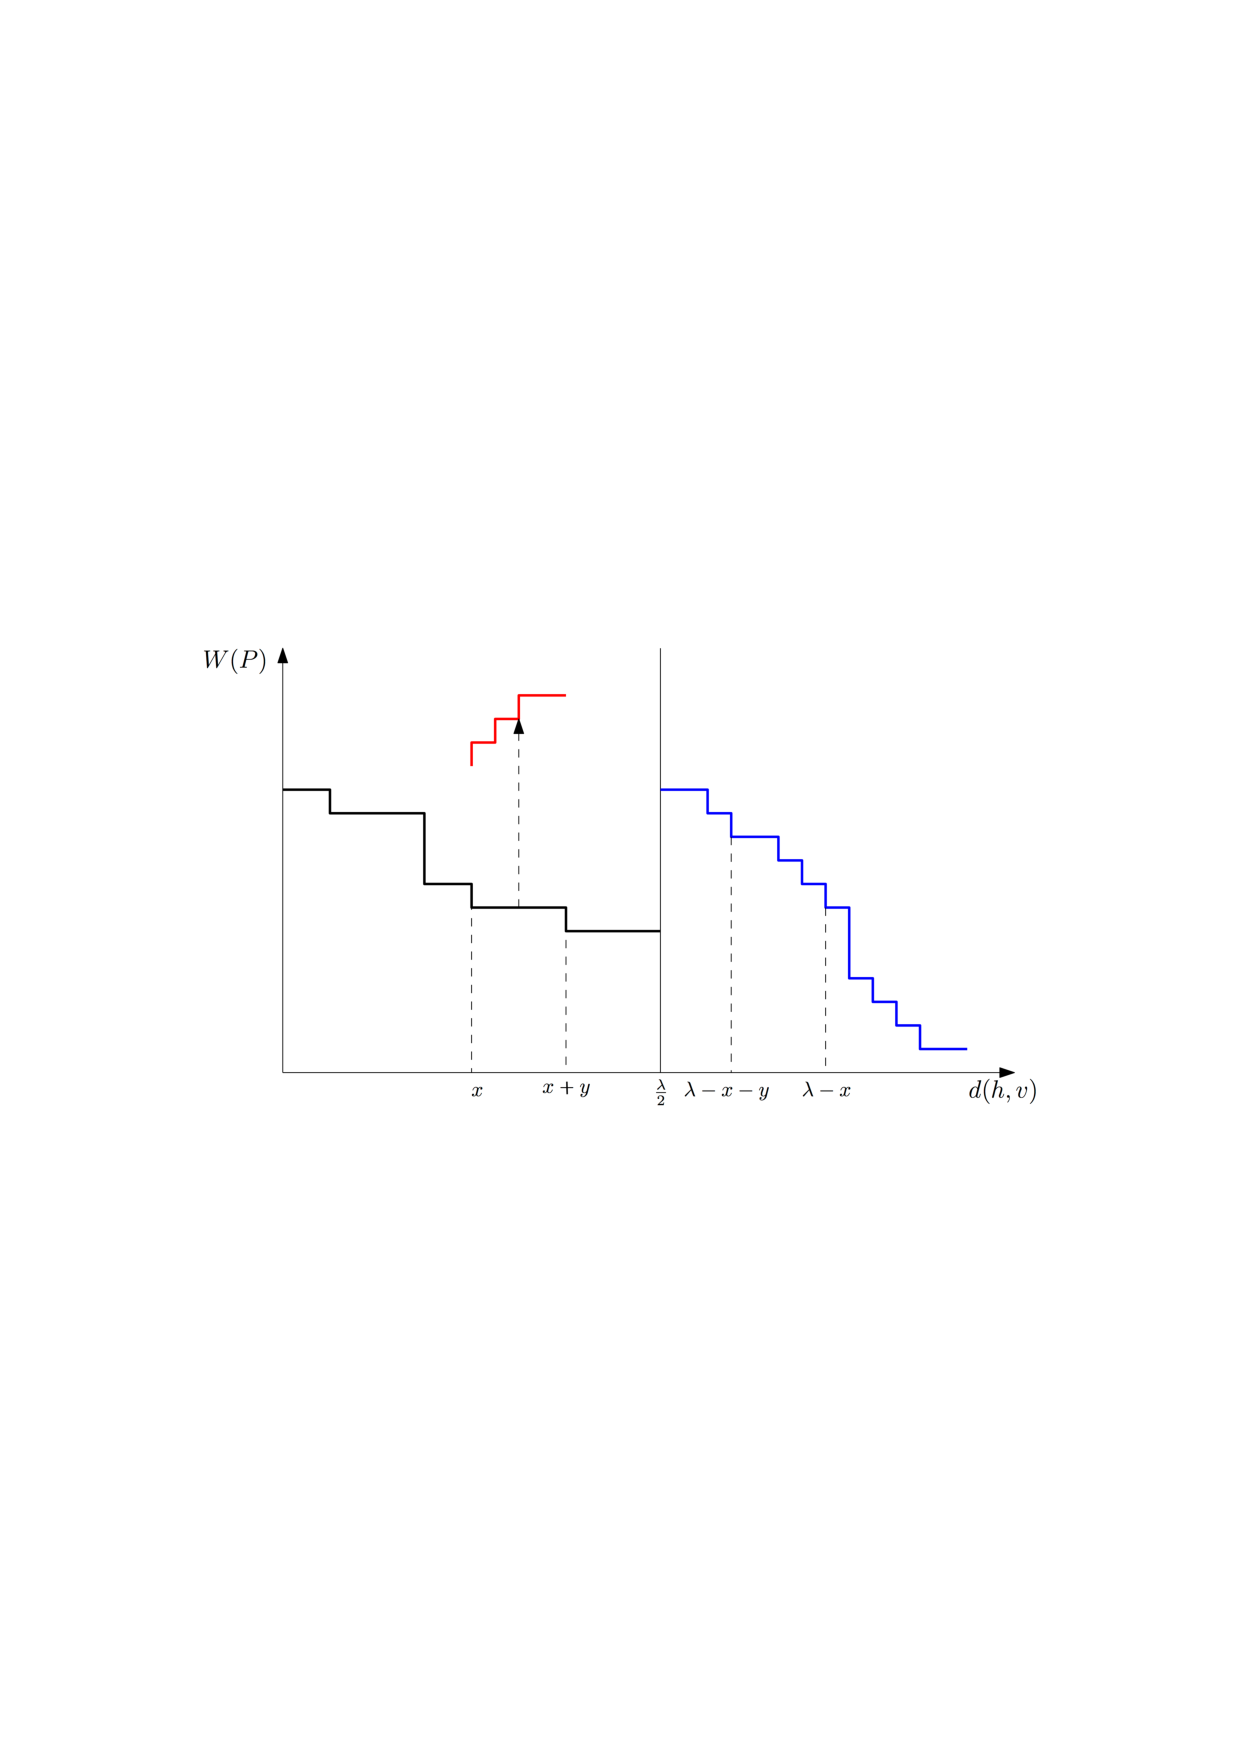
\includegraphics[scale=0.4]{polyline_first_half_construction_case1}
\end{center}
\caption{The first case of constructing the first half of the polyline. $p_1'$ (in blue) is the first half of $p_1$, $p_2'$ (in red) is the second half of $p_2$, mirrored. The black polyline is the result of summing the value of the two polylines for each point, and so it not a monotone polyline.
\label{figure of constructing the second half of the polyline case 1}}
\end{figure}


We now consider the second case, where $d(h_1,v) > d(h_2,v)$ (i.e. the closest chosen node in $v$'s subtree is inside $u_2$'s subtree). This time we would have liked to iterate over the first half of $p_2$ while iterating over the second half of $p_1$ backwards. We split both polylines at $\frac{\lambda}{2}$, take the first half of $p_2$ and the second half of $p_1$. We then increase the intervals of $p_2$ induced by breakpoints of $p_1$ by the appropriate values, similarly to what we did in the first step. Again, the resulting polyline may be non-monotone, but this time we cannot solve the problem as in the previous case, since the number of breakpoints in the resulting polyline can be even larger than the number of breakpoints of $p_2$ in the worst case. In order to make the polyline monotone, we need to delete breakpoints in some intervals of the polyline. These intervals can be found by running \emph{value predecessor} queries. For each key of a breakpoint of $p_1$, $bp$, we find the value of the same key in the new polyline. Denote this value by $y$. We then search for the last point (i.e. the point with maximal key) in the new polyline s.t. its value is greater or equal $y$, and its key is smaller than $bp$ (i.e. a value predecessor query). If this point exist, the value of the new polyline between it and $bp$ should be the same. After finding all such intervals (each of which is defined by a breakpoint of $p_1$, and the point we found), we delete all the breakpoints inside these intervals. This ensures that the resulting polyline is monotone decreasing. %The resulting polyline's number of breakpoints is linear in the number of breakpoints of $p_2$.

\begin{figure}[h]
\begin{center}
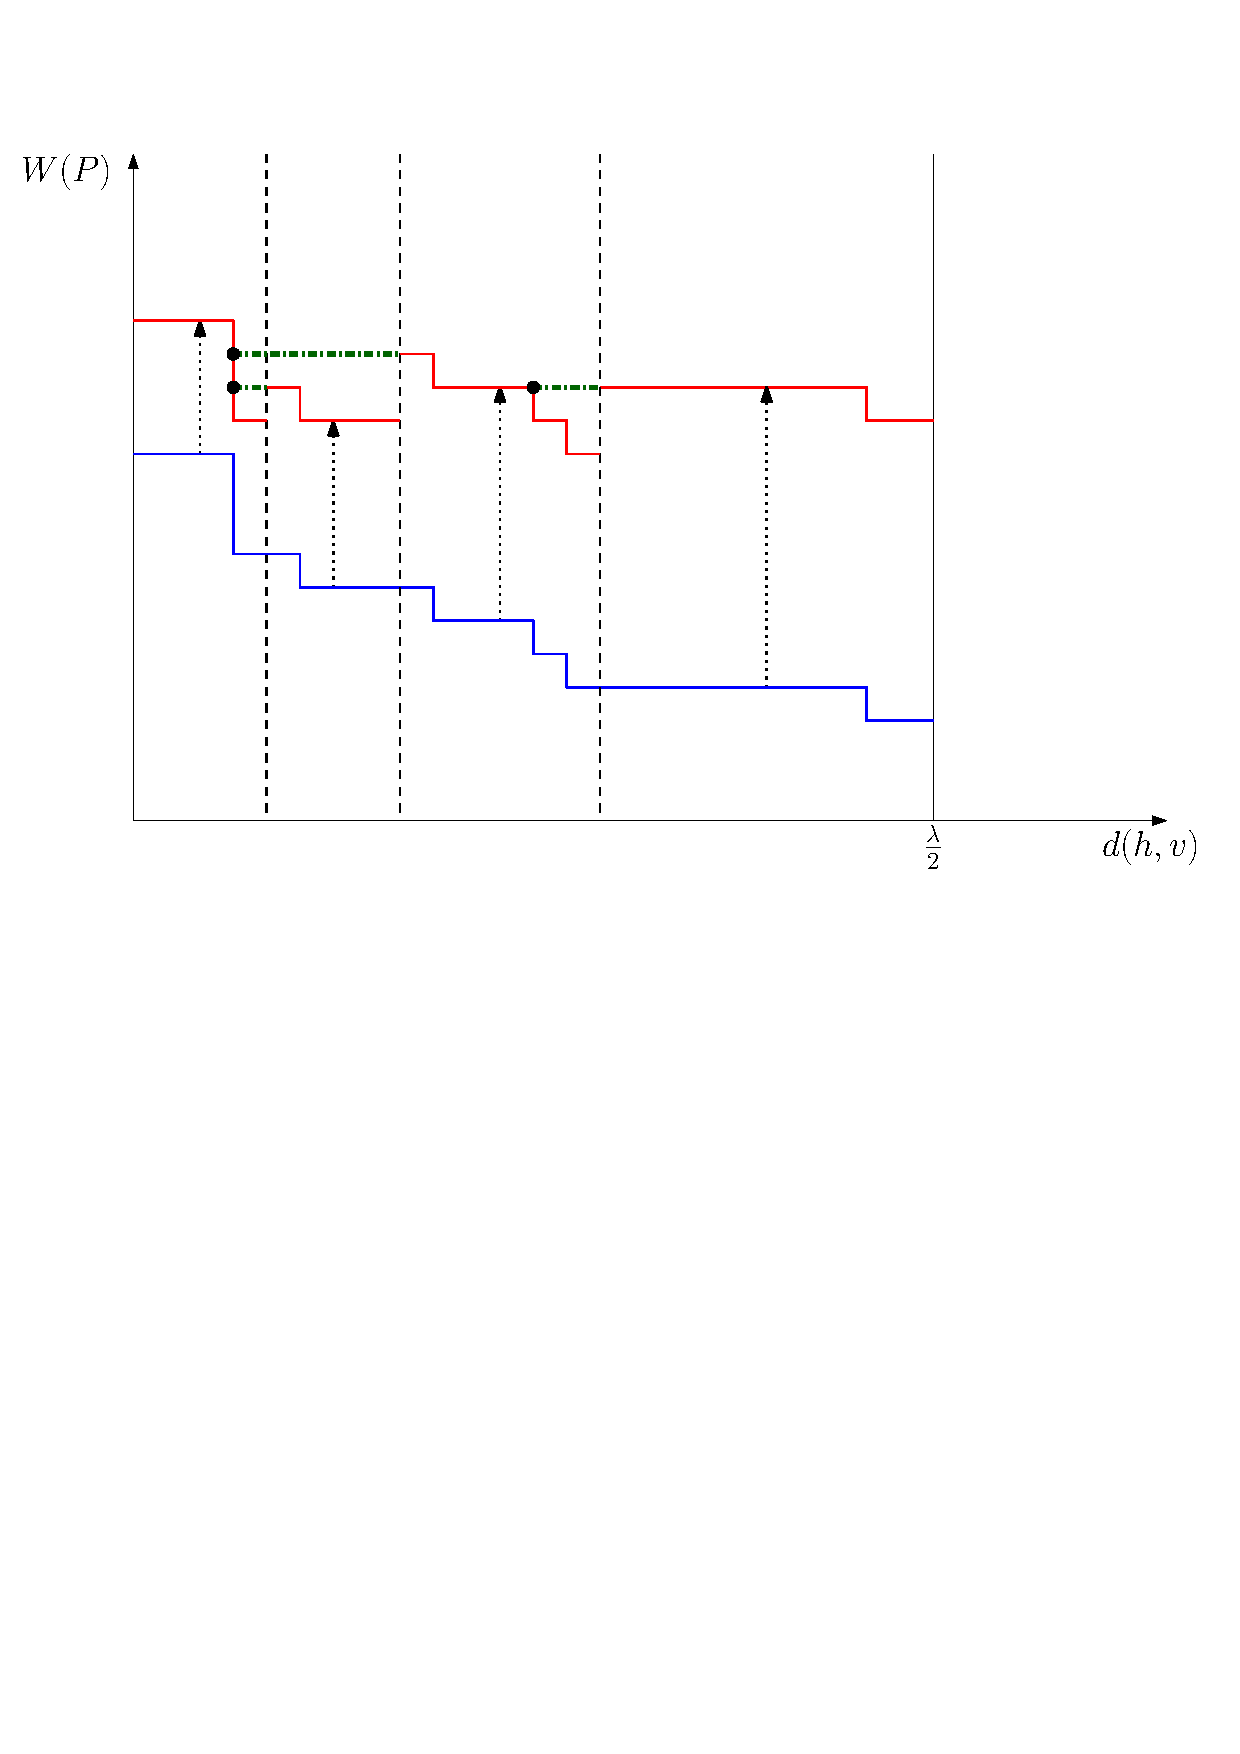
\includegraphics[scale=0.5]{polyline_first_half_construction_case2}
\end{center}
\caption{The second step of constructing the first half of the polyline. The first half of $p_2$ is in blue. The vertical black dashed lines are the breakpoints of $p_1$. We lift the intervals of $p_2$ and get the red polyline, which is not monotone. We delete all the breakpoints in the intervals (in green dashed-dotted lines), and get a monotone decreasing polyline.
}
\end{figure}



%and shift it right by $\lambda$ (since we are interested in $\lambda - d(h_1,v)$)
\end{enumerate}

We now need to build one polyline for the first half of the polyline, taking into account both cases. This is done by taking the maximum of the values of the polylines we just built (denoted by $p_a$ and $p_b$), for every point (s.t. $0 \leq d(h,v) < \frac{\lambda}{2}$). The key is to find the intersection points of the two polylines. Notice that these intersections can only occur at breakpoints of $p_a$, and at most at one point between two consecutive breakpoints of $p_a$. We iterate over the smaller of the two resulting polylines, $p_a$, and for every pair of consecutive breakpoints, we check which polyline has a higher value at both points. If the answer for both points is the same, we carry on. Otherwise, there must be a single intersection point of the two polyline inside this interval (since the two polylines are monotone decreasing). We find this intersection by running a value predecessor query on $p_b$, with the key of the ending point of the interval. In the end of this iteration we know which polyline gives us the best solution for every point between zero and $\frac{\lambda}{2}$, and where are the intersection points where this changes. We can now build the new polyline by doing insertions and deletions in $p_b$, according to the intersection points. For every interval of $p_b$ defined by a pair of consecutive intersection points, we check if the value of $p_a$ is larger than the value of $p_b$ in the interval, and if so, delete all the breakpoints of $p_b$ in the interval, and insert the breakpoints in this interval from $p_a$. This can be viewed as deleting all breakpoints in some list of intervals of $p_b$, and then batched insertions of some breakpoints, between breakpoints of $p_b$ (which are now consecutive, since we deleted the breakpoints that were between them). Since the intersection points can only be at the breakpoints of $p_a$, and at most at one breakpoint of $p_b$ between two consecutive breakpoints of $p_a$, the number of intersection points is linear in the number of breakpoints of $p_a$ (which is linear in the number of breakpoints of $p_1$), and so, the total number of interval deletions and insertions we do is linear in the number of breakpoints of $p_1$. Merging this polyline with the polyline we got for $d(h,v) \geq \frac{\lambda}{2}$ and with the value we have for the case the root is chosen, will give us the polyline representing the solution $P$, for every possible distance of the closest chosen node in $v$'s subtree.

We now need to consider which data structure we will use to store our polylines. The interface we require is:
\begin{enumerate}
\item Shift the polyline right by some distance.
\item Split the polyline at some key.
\item Merge two polylines (s.t. the keys in one polyline are smaller than all keys in the other).
\item "Mirror" a polyline, by negating all the keys ($d(h,v)$) and adding $\lambda$.
\item Query the value of the polyline for a certain key $d(h,v)$.
\item Batched interval increase - Given a list of disjoint intervals of the polyline, and a number for each interval, increase the value of the polyline in each interval by the appropriate number. Each interval is given by the keys of its endpoints.
\item Batched value predecessor - Given a list of key-value pairs, $\{(k_i,v_i)\}$, find for each $k_i$, the maximal key $k_{i}'$, s.t. $k_{i}' \leq k_i$ and the value of the polyline at $k_{i}'$ is larger or equal to $v_i$.
\item Batched interval insertions - Given a list of pairs of consecutive breakpoints in the polyline, insert between each pair a list of breakpoints.
\item Batched interval deletions - Given a list of disjoint intervals of the polyline, delete all the breakpoints inside the intervals.
\end{enumerate}

We now show how to use some standard techniques to implement the required operations, and achieve $O(n \log ^2 n)$ time for our weighted feasibility test. In the next section we will use some more advanced techniques, which allow us to implement the operations more efficiently, and lower the overall running time of our algorithm.

We represent the polylines by storing their breakpoints in augmented B Trees, where the data is stored in the leaves. Each node of the trees will store a key-value pair. The breakpoints of the polyline will be stored at the leaves of the tree, and we will maintain the following property: the key of each leaf will be the sum of the keys of all its ancestors, and its value will be the sum of the values of all its ancestors.

Let us describe the implementation of each operation. We denote the number of breakpoints in $p_1$ (the smaller polyline) by $x$, and the number of breakpoint of $p_2$ by $y$ (i.e. $x \leq y$). Operation 1 can simply be implemented by adding the required distance to the key at the root of the tree. This will take constant time. Operations 2 and 3 can use standard split and merge procedures for balanced search trees. This will take logarithmic time. Operation 4 requires saving an extra bit in the root of the tree, thus allowing to negate all the keys in the tree by switching it (all the procedures will switch right and left when the negation flag is on). After the negation, the mirroring operation will add $\lambda$ to all the keys in the tree (by adding to the root). This is done in constant time. Operation 5 can be done by a predecessor query, and returning the value at the previous breakpoint.

Operations 1-5 are performed only a constant number of times per step, and so their total cost is logarithmic. The next four operations are the more costly, since each of the them is comprised of a batch of $O(x)$ operations on a tree of size $O(y)$.

Operation 6 - batched interval increase: we iterate over the intervals and for each interval, we traverse the tree from the starting point of the interval, through the LCA, and to the ending point of the interval. We store in each node of the tree the maximum of its subree, so we know when we reach the LCA. On the way up to the LCA we increase the key of every right child which is not on the path, and on the way down from the LCA we increase the key of every left child that is not in the path. This operation take time which is linear in the number of nodes reached by the described traversal. Since we use a balanced tree, the distance between interval endpoints and their LCA is at $O(\log y)$, and so the operation takes $O(x \log y)$ in the worst case.

Operation 7 - batched value predecessor: We store in each node the maximum value in its subtree. Each value predecessor query will be answered by first finding $k_i$ (or it's predecessor, if there is no breakpoint at $k_i$). Then we go up the tree until the maximum value in at least one subtree rooted at one of the current node's children (other than the child from which we came) is larger or equal to the value of the starting point. Then we go down while searching for the right-most leaf which has value at least $v_i$. This search is done by always going down to the right-most child that has such a leaf in its subtree. Each predecessor key takes $O(\log y)$ and so the operation takes $O(x \log y)$ in total.

Operation 8 - Batched interval insertions: In this section, it is enough to simply insert the nodes one by one, with the standard insertion procedure which works in logarithmic time. The operation takes $O(x \log y)$ in total.

Operation 9 - Batched interval deletions: Again, the standard deletion procedure is good enough at this point, and the operation takes $O(x \log y)$ time.
 
\begin{lemma}
The above implementation induces $O(n \log ^2 n)$ complexity for our weighted feasibility test.
\end{lemma}

\begin{proof}
Notice that the number of breakpoints in a polyline representing some subtree, is at most the number of nodes in the same subtree. This is because in each breakpoint we have a decreae in the weight of the solution, due to some node that could have been in the solution for smaller keys of the polyline, but is now too close to the root. This node will not be in the solution for any key after this breakpoint.

The running time of the algorithm is the sum of running times required for constructing the polyline of the subtree rooted at each node of the tree. We split the analysis into two parts: first we consider nodes of degree one, and then nodes of degree two.
For any node with degree one, constructing the polyline for its subtree, given the polyline for the subtree rooted at its child takes logarithmic time, i.e. no more than $O(\log n)$. Since we have at most $n$ nodes with degree one, the total processing time for these nodes is $O(n \log n)$.
 
As we mentioned, operations 1-5 only take logarithmic time per step, while operations 6-9 take $O(x \log y)$ time.  Thus, constructing the polyline for the subtree rooted at some node $v$, with degree two, takes $O(x \log y)$ time, where $x$ and $y$ are the sizes of the subtrees rooted at the children of $v$, and $x \leq y$. Clearly it holds that $x \log y \leq x \log n$, so the total running time for all nodes with degree two is bounded by $S \cdot \log n$, where $S$ is the sum of sizes of the smaller subtrees for all nodes of degree two.

We prove by induction that for any binary tree with $n$ nodes, $S \leq n \log n$. It easy to see that the base of the induction holds. Assume that for any binary tree with $k$ nodes, where $k<n$, it holds that $S \leq k\log k$. Consider some binary tree with $n$ nodes. If the root of the tree has only one child, $S$ is the same for the subtree rooted at the child, and so $S \leq (n-1)\log (n-1) < n \log n$. If the root has two children, denote the size of its left subtree by $x$ and the size of its right subtree by $y$ so that $n=1+x+y$. Assume w.l.o.g. that $x \leq y$. From the induction hypothesis it follows that $S \leq x + x \log x + y \log y$. We would like to prove that $x + x \log x + y \log y \leq n \log n$. This holds because:
\begin{align*}
x + x\log x + y\log y &= x \log (2x) + y\log y \\
& \leq x \log (x+y) + y\log y \\
& \leq x \log (x+y) + y \log (x+y) \\
& = (x+y)\log(x+y) < n \log n.
\end{align*}
We conclude that the total complexity of our weighted feasibility test is $O(n \log n \cdot \log n) = O(n \log ^2 n)$.
\end{proof}


\subsection{An \boldmath$O(n \log n)$ Algorithm for the weighted feasibility test}
We now present an optimal $O(n \log n)$ time algorithm for the weighted feasibility test. We use the same algorithm described in the previous section, and reduce its running by implementing the heavier operations we run on the polylines more efficiently. Previously, we had a running time of $O(x \log y)$ for these operations, and we will now show how we can reduce this to $O(x \log (\frac{y}{x}))$ time per operation, which will induce a running time of $O(n \log n)$ for the entire algorithm. We achieve this running time by using properties of Finger Search Trees proven by Huddelston and Melhorn In. %TODO cite. 
In this section we use $(2,5)$ Trees to store our polylines.
The main idea we use is analysing the complexity of operations more carefully, by looking at the performance of the basic operations we do on our balanced trees (i.e. search, insert and delete) in the context of the interface we defined, and what we do in each step of the algorithm (i.e. the batched operations). We will show that since these basic operations are not performed in random, the amortized cost of each operation is less than logarithmic.

Our four batched operations traverse the search tree in the same way. Given a list of $x$ leaves we, denoted by $p_1,p_2,...,p_x$, define an \emph{interval traversal} on these leaves as a traversal on the path $r \rightarrow p_1 \rightarrow p_2 \rightarrow ... \rightarrow p_x$ (where $r$ is the root of the tree). 
%For $1 \leq i \leq x$, and to get from one leaf to the next, we go up to their LCA, and then go down. %TODO add figure
\begin{lemma} \label{interval traversal lemma}
The number of nodes in an interval traversal over $O(x)$ leaves in a tree with $O(y)$ leaves is $O(x \log (\frac{y}{x}))$,
\end{lemma}
\begin{proof}
Theorem 4 in %TODO cite.
shows that the number of different ancestors of $x$ leaves in a $(a, \infty)$ with $y$ leaves, is at most $3x + 2( \log _{a}{y} + \sum_{i=2}^{x} \log (d_i))$, where $d_i$ is the number of leaves in the tree that are between $p_{i-1}$ and $p_i$. The lemma is implied directly from this, due to convexity of the logarithm function.
\end{proof}

By Lemma \ref{interval traversal lemma}, the running time of operations 6 and 7 is $O(x \log (\frac{y}{x})$, since their running time is linear in the number of nodes traversed by them.



\bibliographystyle{abbrv}
\bibliography{dispersion}

\end{document}